% LaTeX-Vorlage
% mit ein paar n�tzlichen Abk�rzungen
%
% Autor:
\author{Stefan~Hedinger}
% Datum: heute  
\date{\today}
% Versionsnummer: 
\newcommand{\versionsnummer}{1.0}

% Titel: 
\title{Analog Microelectronics \\[1ex] \large Nach der Vorlesung von Prof. Dr. Paul Zbinden (FS2016)\\[2ex] \small Version: \versionsnummer}
%
% DIN A4 Seite: 
\documentclass[10pt,a4paper]{article}
% viele packages: 
% (die, die man nicht benötigt, kann weglassen)
\usepackage{ngerman}
\usepackage{curves}
\usepackage{latexsym} % ein paar Symbole
\usepackage{textcomp} % ein paar Symbole
\usepackage{amsfonts}
\usepackage{siunitx}  % SI Einheiten
\usepackage{ulem} 
\usepackage[dvips]{rotating} % für rotate-Befehl
\usepackage[utf8]{inputenc}
%\usepackage[latin1]{inputenc} 
\usepackage{geometry}
% 
% Seitengeometrie festlegen:
\geometry{left=1.5cm,textwidth=19cm,top=2cm,textheight=26cm}
%
% header & footer
\usepackage{fancyhdr}
\pagestyle{fancy}
\fancyhf{}
\fancyhead[L]{AnME}
\fancyhead[C]{\leftmark}
\fancyhead[R]{\thepage}
\renewcommand{\headrulewidth}{0.4pt}
\fancyfoot[L]{Stefan Hedinger}
\fancyfoot[C]{\small{Dieses Dokument wurde mit \LaTeX{} erstellt.}}
\fancyfoot[R]{\today}
\renewcommand{\footrulewidth}{0.4pt}
%\usepackage[draft]{graphics} % ohne Bilder (Entwurf)
% Figures
\usepackage{pdfpages}
\usepackage{epstopdf}
\usepackage{float}
\usepackage{wrapfig}
\usepackage[export]{adjustbox}
\usepackage{graphics} % Bilder einbinden
\nonfrenchspacing
%
% Abkürzungen
\newcommand{\nach}{\, \mathrm{d}} % Zeichen f�r z.B. "Integral ... nach x"
\newcommand{\divergenz}{\, \mathrm{div} \,} % Divergenz
\newcommand{\grad}{\, \mathrm{grad} \,} % Gradient
\newcommand{\rot}{\, \mathrm{rot} \,} % Rotation
\newcommand{\laplace}{\Delta} % Laplace-Operator
\newcommand{\arccot}{\, \mathrm{arccot} \,}
\newcommand{\arsinh}{\, \mathrm{arsinh} \,}
\newcommand{\arcosh}{\, \mathrm{arcosh} \,}
\newcommand{\artanh}{\, \mathrm{artanh} \,}
\newcommand{\arcoth}{\, \mathrm{arcoth} \,}
\newcommand{\sgn}{\, \mathrm{sgn} \,}  % Signumfunktion
%\newcommand{\si}{\, \mathrm{si} \,}  % si(x) = sin(x)/x
\newcommand{\ld}{\, \mathrm{ld} \,}  % Logarithmus zur Basis 2
\newcommand{\Si}{\, \mathrm{Si} \,}  % Integral von si(x)
\newcommand{\f}{\, \mathrm{f} \,}  % all. Funktion
\newcommand{\s}{\, \mathrm{s} \,}  % Sprung-Funktion
\newcommand{\kz}{\! \times \!}  % Vektor-Kreuzprodukt
\newcommand{\trafo}{\enspace\circ\!\!-\!\!\bullet\enspace} % Zeichen f�r "Transformierte von"
\newcommand{\rtrafo}{\enspace\bullet\!\!-\!\!\circ\enspace} % Zeichen f�r "R�cktransformierte von"
\newcommand{\vint}{\int\!\!\int\limits_V\!\!\int} % Volumenintegral
\newcommand{\vstrichint}{\int\!\!\int\limits_{V'}\!\!\int} % gestrichenes Volumenintegral
\newcommand{\aint}{\int\limits_a\!\!\int} % Fl�chenintegral
\newcommand{\astrichint}{\int\limits_{a'}\!\!\int} % gestrichenes Fl�chenintegral
\newcommand{\aoint}{\oint\limits_a\!\!\!\!\int} % Fl�chenh�llintegral  %+++ keine gute L�sung ! 
\newcommand{\aostrichint}{\oint\limits_{a'}\!\!\!\!\int} % gestrichenes 	Fl�chenh�llintegral  %+++ keine gute L�sung ! 
\newcommand{\sint}{\int\limits_s} % Wegintegral
\newcommand{\sstrichint}{\int\limits_s} % gestrichenes Wegintegral
\newcommand{\soint}{\oint\limits_s} % geschlossenes Wegintegral
\newcommand{\lint}{\int\limits} % Integral mit den Grenzen ...
\newcommand{\lsum}{\sum\limits} % Summe mit den Grenzen
\newcommand{\llim}{\lim\limits} % Limes
\newcommand{\olint}{\oint\limits} % H�llintegral �ber ...
\newcommand{\intinfty}{\int\limits_{-\infty}^{\infty}} % Integral von Plus bis Minus unendlich
\newcommand{\suminfty}{\sum\limits_{n=-\infty}^{\infty}} % Summe von Plus bis Minus unendlich
\newcommand{\gefaltet}{\ast} % Faltung zweier Funktionen
\newcommand{\bild}[2]{\raisebox{-0.4\height}{\resizebox{!}{#2}{\includegraphics{grafiken/#1}}}} %Grafiken einbinden (z.B. .eps-Dateien)
\newcommand{\mod}{\, \mathrm{mod} \,} % Modulo-Operator
\newcommand{\V}{\left(\begin{array}{c}} % Vektor 
\newcommand{\Vend}{\end{array}\right)}  % Vektorende
% damit kann man einen Vektor einfach so schreiben : "\V 5 \\ 3 \\ 7 \Vend"
\newcommand{\sollgleich}{\raisebox{1ex}{\(!\atop =\)}} % soll gleich ... sein
\newcommand{\bul}{\textbullet \quad} % Aufz�hlungspunkt, 1. Ebene
\newcommand{\bull}{\textopenbullet \quad} % Aufz�hlungspunkt, 2. Ebene
\newcommand{\heraus}{\(\bigodot\)} % Fluss aus der Bildebene heraus
\newcommand{\hinein}{\(\bigotimes\)} % Fluss in die Bildebene hinein
\newcommand{\kleinhinein}{\(\otimes\)} % Fluss in die Bildebene hinein
\newcommand{\nicht}{\overline} % logische Negation (Strich ueber dem Symbol, ist besser lesbar als \bar)
\newcommand{\vereinigt}{\cup} % Symbol: Vereinigung aus 2 Mengen
\newcommand{\geschnitten}{\cap} % Symbol: Schnittmenge aus 2 Mengen
\newcommand{\complement}{^c} % Symbol f�r Komplement�rmenge
\newcommand{\aequivalent}{\quad \( \Leftrightarrow \) \quad} % �quivalenz
\newcommand{\cv}{\, \mathrm{cv} \,} % Variationskoeffizent
\newcommand{\var}{\, \mathrm{var} \,} % Varianz
\newcommand{\cov}{\, \mathrm{cov} \,} % Kovarianz
\newcommand{\geom}{\, \mathrm{geom} \,} % geometrische Verteilung
\newcommand{\und}{\enspace \mathrm{\wedge} \enspace} % log. "und"
\newcommand{\oder}{\enspace \mathrm{\vee} \enspace} % log. "oder"
\newcommand{\C}{\textnormal{\small I}\!\!\!\mathbf{C}} %Zeichen f�r Menge der Komplexen Zahlen
\newcommand{\N}{\mathbf{I}\!\!\!\mathbf{N}} %Zeichen f�r Menge der nat�rlichen Zahlen
\newcommand{\R}{\mathbf{I}\!\!\!\mathbf{R}} %Zeichen f�r Menge der reellen Zahlen
\newcommand{\ueber}{\choose} % "�ber" z.B. f�r Binominalkoeffizenten
%
\begin{document}
%
% Titelseite:
\maketitle
%
% Inhaltsverzeichnis : (wird beim 2. mal compilieren automatisch erstellt)
\setcounter{tocdepth}{2}
\tableofcontents
%

%
%\newpage
%
% !TeX spellcheck = de_CH_frami

\section{CMOS Technologie (Kap. 3)}

\begin{minipage}[t]{0.5\textwidth}
	\textbf{Oberflächenbeschichtung}\\
	Epitaxie, Oxidation oder Abscheideverfahren\\ [2ex]
	\textbf{Fotolithografie}\\
	Auftragen von Fotolack, anschliessend belichten\\ [2ex]
	\textbf{Ätzen}\\
	Abtragen der Beschichtung
	\begin{figure}[H]
		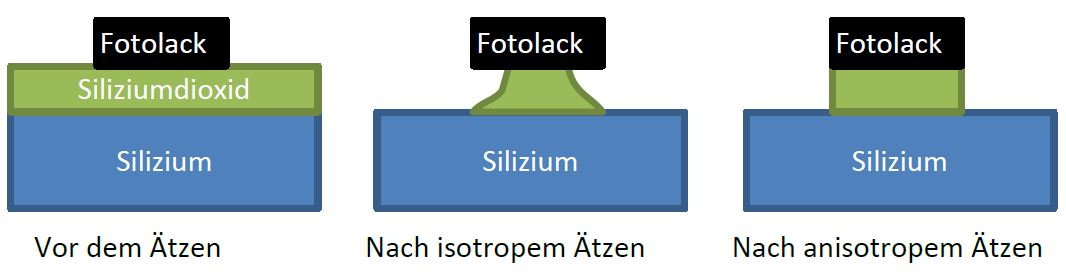
\includegraphics[width=0.8\linewidth]{chapters/Technologie/images/Aetzen}
	\end{figure}
	\begin{tabular}{|l|l|}
		\hline
		\textbf{Bezeichnung}&\textbf{Ätzverfahren}\\ \hline
		Isotropes Ätzen&nasschemisches Ätzen\\ \hline
		Anisotropes Ätzen&Plasmaätzen\\ \hline
	\end{tabular}\\ [2ex]
	\textbf{Dotieren}\\
	Anschluss der Schicht erstellen\\ [2ex]
	\textbf{Säubern der Wafer}\\
\end{minipage}
\begin{minipage}[t]{0.5\textwidth}
	\textbf{Ablauf CMOS Herstellungsprozess}\\
	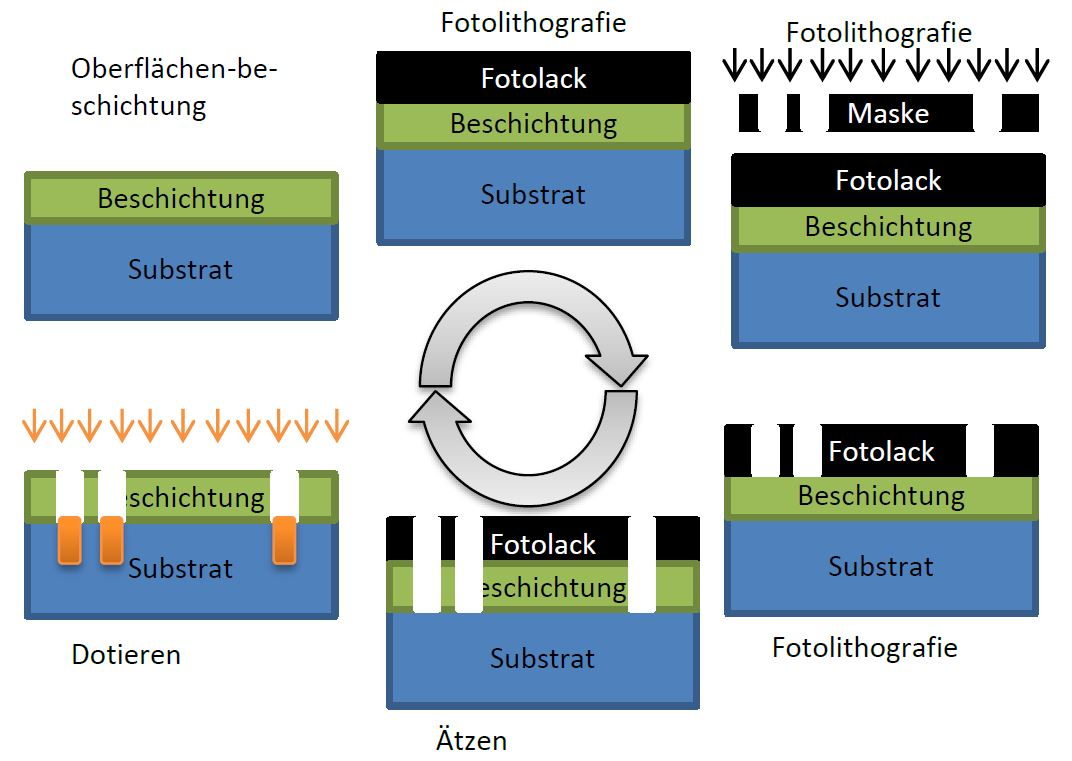
\includegraphics[width=1\textwidth, right]{chapters/Technologie/images/Verarbeitung}
	\textbf{CMOS Technologie - Dotierung}\\ 
	\begin{tabular}{|l|l|l|}
		\hline
		\textbf{Wertigkeit}&\textbf{Dotierung}&\textbf{Material}\\ \hline
		3&p&Bor (B)\\ \hline
		4&-&Silizium (Si)\\ \hline
		5&n&Arsen (As)\\ \hline
	\end{tabular}
\end{minipage}

\section{Passive Schaltungselemente in CMOS (Kap. 4)}

\begin{minipage}[c]{0.22\textwidth}
	Absolute Genauigkeit:\\Relative Genauigkeit:
\end{minipage}
\begin{minipage}[c]{0.06\textwidth}
	$\pm \SI{20}{\percent}$\\ $\pm \SI{1}{\percent}$
\end{minipage}
\begin{minipage}[c]{0.5\textwidth}
	(Wert vom einzelnen Element)\\(Verhältnis von Elementen zueinander)
\end{minipage}\\[1ex]
Da Verhältnisse sehr genau sind, werden sie in der Schaltungstechnik intensiv genutzt.

\subsection{Kapazitäten}
Auf einem Chip bilden sich zwischen zwei voneinander isolierten Elektroden Kapazitäten.
\\[2ex]
\begin{minipage}[c]{0.55\textwidth}
	\begin{tabular}{|l|l|}
		\hline
		Poly-Poly-Kapazität ($Si$-$SiO_2$-$Si$) & $C'' \approx \SI{1}{\femto \farad \per \micro \meter ^2}$\\ \hline
		MOS-Kapazität (Gate-Gateoxid-Kanal) & $C'' \approx \SI{10}{\femto \farad \per \micro \meter ^2}$\\ \hline
		MIM-Kapazität (Metall-Isolator-Metall) & $C'' \approx \SI{1}{\femto \farad \per \micro \meter ^2}$ \\ \hline
	\end{tabular}
\end{minipage}
%\begin{minipage}[c]{0.35\textwidth}
%	Poly-Poly-Kapazität ($Si$-$SiO_2$-$Si$)\\
%	MOS-Kapazität (Gate-Gateoxid-Kanal)\\
%	MIM-Kapazität (Metall-Isolator-Metall)
%\end{minipage}
%\begin{minipage}[c]{0.2\textwidth}
%	$C'' \approx \SI{1}{\femto \farad \per \micro \meter ^2}$\\
%	$C'' \approx \SI{10}{\femto \farad \per \micro \meter ^2}$\\
%	$C'' \approx \SI{1}{\femto \farad \per \micro \meter ^2}$
%\end{minipage}
\begin{minipage}[c]{0.45\textwidth}
	\uline{\textbf{Legende:}}\\
	$C''$: spezifische Kapazität pro Flächeneinheit\\
	$d$:   Plattenabstand (meist durch Herstellung gegeben)
	%
\end{minipage}
\\[2ex]
\begin{minipage}[c]{0.55\textwidth}
	\uline{\textbf{Formeln:}}\\
	Kapazität/Fläche: $C'' = \frac{\epsilon}{d} = \frac{\epsilon_0 \cdot \epsilon_r}{d}$\\
	Kapazität: \hspace{11.5mm}$C = C'' \cdot A$
\end{minipage}
\begin{minipage}[c]{0.45\textwidth}
	\uline{\textbf{Konstanten:}}\\
	$\epsilon_0 = 8.85 \cdot 10^{-12} \SI{}{\farad / \meter}$\\
	$\epsilon_r = \SI{3.9}{}$ (für Siliziumoxid)
\end{minipage}
\\[2ex]
Neben der gewünschten Kapazität hat jeder Plattenkondensator auch unerwünschte Streukapazitäten. 
Beim Chip fällt vor allem die Streukapazität zwischen der unteren Elektrode und dem Substrat ins Gewicht.

\subsection{Widerstände}
Unerwünscht auf dem Chip, da hoher Platzbedarf und Wärmeentwicklung.
\\[2ex]
\begin{minipage}[c]{0.55\textwidth}
	\begin{tabular}{|l|l|}
		\hline
		Poly-Widerstand & $R_\square \approx \SI{10}{\Omega \per}\square$\\ \hline
		HR-Poly-Widerstand & $R_\square \approx \SI{1}{\kilo\Omega \per}\square$\\ \hline
		P-Diffusions-Widerstand & $R_\square \approx \SI{100}{\Omega \per}\square$\\ \hline
		N-Diffusions-Widerstand & $R_\square \approx \SI{100}{\Omega \per}\square$\\ \hline
		N-Well-Widerstand & $R_\square \approx \SI{1}{\kilo\Omega \per}\square$\\ \hline
	\end{tabular}
\end{minipage}
%\begin{minipage}[c]{0.22\textwidth}
%	Poly-Widerstand\\HR-Poly-Widerstand\\P-Diffusions-Widerstand\\N-Diffusions-Widerstand\\N-Well-Widerstand
%\end{minipage}
%\begin{minipage}[c]{0.33\textwidth}
%	$R_\square \approx \SI{10}{\Omega \per}\square$\\
%	$R_\square \approx \SI{1}{\kilo\Omega \per}\square$\\
%	$R_\square \approx \SI{100}{\Omega \per}\square$\\
%	$R_\square \approx \SI{100}{\Omega \per}\square$\\
%	$R_\square \approx \SI{1}{\kilo\Omega \per}\square$
%\end{minipage}
\begin{minipage}[c]{0.45\textwidth}
	\uline{\textbf{Legende:}}\\
	$R_\square:$ spezifischer Widerstand einer quadratischen Fläche\\\\
	\uline{\textbf{Formel:}}\\
	$R = R_\square \cdot \frac{L}{W}$
\end{minipage}
\\[2ex]
Jeder Widerstand auf dem Chip erzeugt zwangsläufig Streukapazitäten, die es im Design zu berücksichtigen gilt.

\subsection{Induktivitäten}
Mit Standard CMOS-Technologie lassen sich Induktivitäten nicht gut herstellen.
Für RF-Anwendungen werden Spulen eingesetzt, die aber in der Ebene gewickelt werden.
Spulen lassen sich ausserhalb des Chips mit z.B. Bonddrähten realisieren.
% !TeX spellcheck = de_CH_frami

\section{MOS-Transistoren (Kap. 5)}

\begin{minipage}[c]{0.54\textwidth}
	\textbf{Bulk-Anschluss}\\
	Wenn der Bulk-Anschluss nicht gezeichnet ist, gilt die Konvention, dass der Bulk des n-Transistors immer mit VSS und derjenige des p-Transistors immer mit VDD verbunden ist.
	\subsection{Bestimmung des Arbeitsbereichs}
	1. Bestimmung ob weak, moderate oder strong inversion.\\
	2. Berechnen der Sättigungsspannung.\\
	3. Wenn $\mid V_{DS}\mid > \mid V_{DS,sat}\mid$ = gesättigt
\end{minipage}
\begin{minipage}[c]{0.13\textwidth}
	\uline{\textbf{NMOS:}}\\
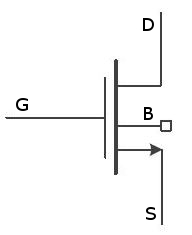
\includegraphics[width=1\textwidth]{chapters/Transistoren/images/N-MOS}
\end{minipage}
\begin{minipage}[c]{0.13\textwidth}
	\uline{\textbf{PMOS:}}\\
	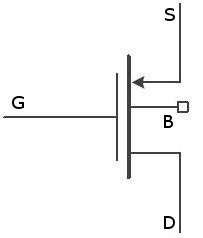
\includegraphics[width=1\textwidth]{chapters/Transistoren/images/P-MOS}
\end{minipage}
\begin{minipage}[c]{0.2\textwidth}
	\textbf{Legende:}\\
	G: Gate\\
	D: Drain\\
	S: Source\\
	B: Bulk
\end{minipage}
\\[2ex]
\begin{minipage}[c]{0.76\textwidth}
	\begin{tabular}{|l|l|l|}
		\hline
		\textbf{Arbeitsbereich}& \textbf{Bedingung} & \textbf{Sättigungspannung}\\ \hline
		weak inversion& $0 < V_{GS} < V_T - \SI{60}{\milli\volt}$ & $V_{DS,sat}\approx 5\Phi _t \approx \SI{130}{\milli\volt}$ \\
		& &(bei $T = \SI{300}{\kelvin} = \SI{27}{\degreeCelsius}$) \\
		$I'_D < I'_M$& & $V_{GS} = V_M +n_M \cdot \Phi_t \cdot \ln{\frac{I_D}{\frac{W}{L}\cdot I_M}}$\\ \hline
		moderate inversion& $V_T - \SI{60}{\milli\volt} < V_{GS} < V_T + \SI{160}{\milli\volt} $ & \\
		$I'_M < I'_D < I'_H$& & \\ \hline
		strong inversion& $V_T + \SI{160}{\milli\volt} < V_{GS}$ & $V_{DS,sat} = V_{GS}-V_T = \sqrt{\frac{2I_D}{\beta}}$\\
		$I'_H < I'_D$& & \\ \hline
	\end{tabular}
\end{minipage}
\begin{minipage}[c]{0.24\textwidth}
	\uline{\textbf{Formeln:}}\\
	$I_D = \frac{W}{L}\cdot I'_D$\\
	$\Phi_t = V_{temp} = \frac{k\cdot T}{e}$\\
	$\Phi_t = \SI{25.9}{\milli\volt}$ @ $T = \SI{27}{\degreeCelsius}$\\
	$\beta = \frac{W}{L} \cdot \beta_0$ \\[2ex]
	\uline{\textbf{Konstanten:}}\\
	$k = \SI{1.38e-23}{\joule /\kelvin}$\\
	$e = \SI{1.60e-19}{\coulomb}$
\end{minipage}

\subsection{Kennlinien}
\subsubsection{Ausgangskennlinie}

\begin{minipage}[c]{0.35\textwidth}
	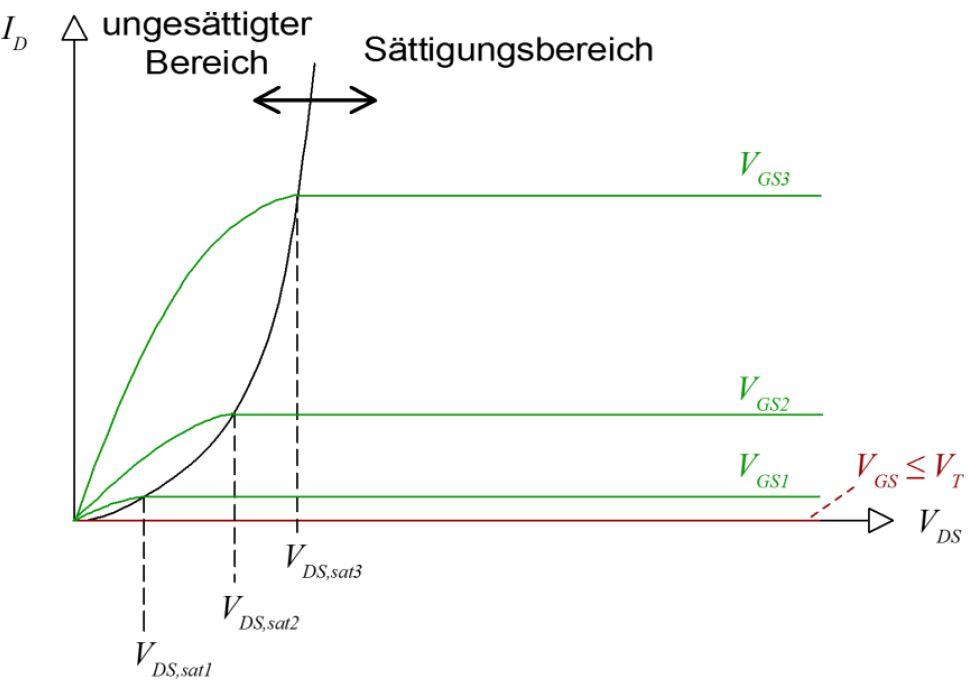
\includegraphics[width=1\linewidth]{chapters/Transistoren/images/Ausgangskennlinie}
\end{minipage}
\begin{minipage}[c]{0.65\textwidth}
	\textbf{Gesättigt}, Stromquellen-Betrieb:\\
	Geraden horizontal, dann ist $r_{DS} = \infty$ (idealer Transistor).\\
	Anstieg der Geraden entspricht Ausgangsleitwert $g_o$ o. Ausgangswiderstand $r_{DS}$\\
	$r_{DS} = \frac{1}{g_o} = \frac{dV_{DS}}{dI_D} \approx \frac{\Delta V_{DS}}{\Delta I_D}$\\ \\
	\textbf{Ungesättigt}, Widerstandsbetrieb:\\
	Je steiler die Gerade, desto kleiner $r_{DS}$
\end{minipage}

\subsubsection{Transferkennlinie}
\begin{minipage}{0.4\textwidth}
	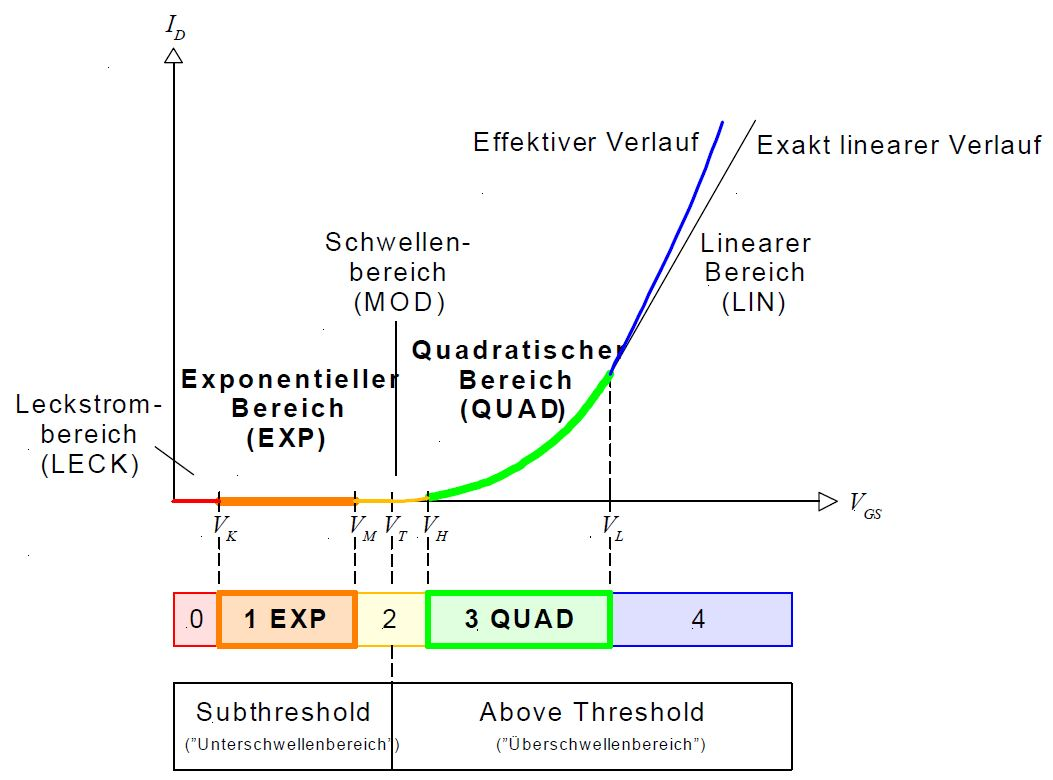
\includegraphics[width=1\linewidth]{chapters/Transistoren/images/Transferkennlinie}
\end{minipage}
\begin{minipage}{0.6\textwidth}
	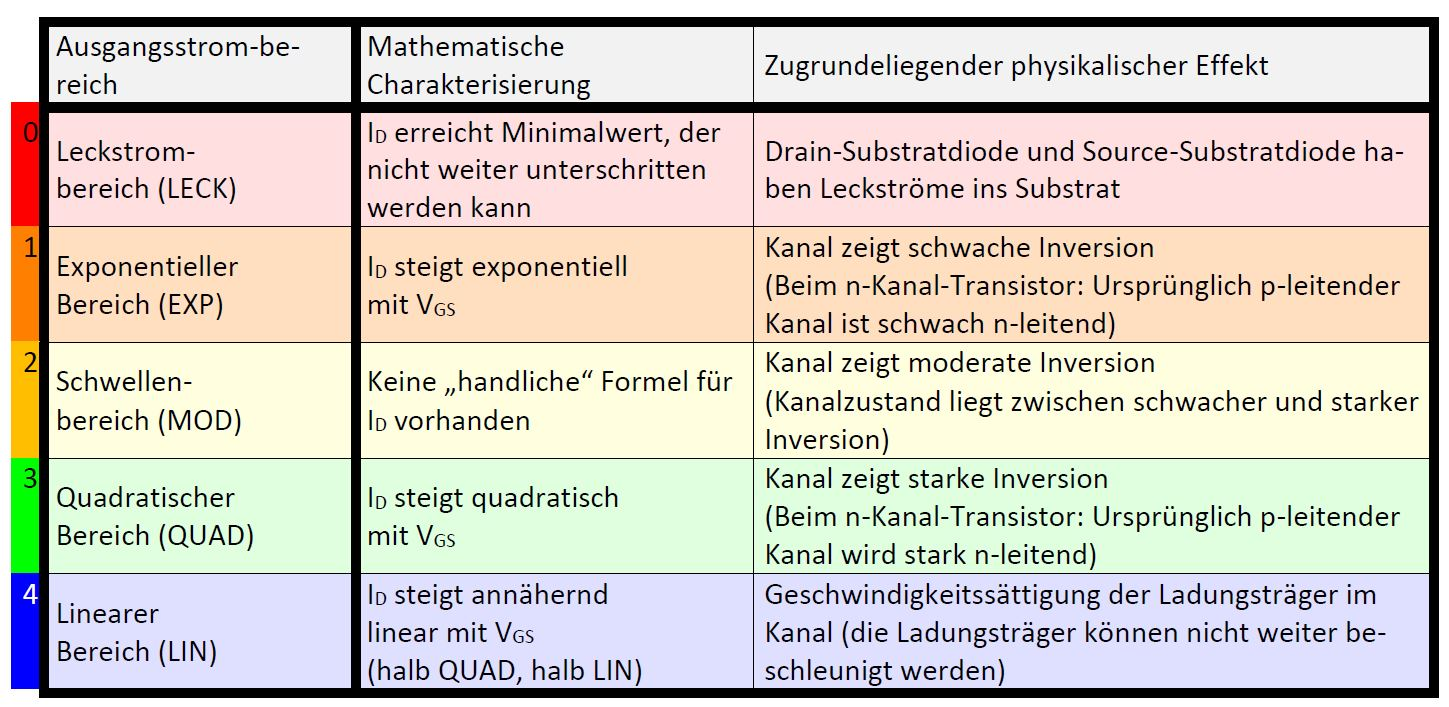
\includegraphics[width=1\linewidth]{chapters/Transistoren/images/Ausgangsstrombereich} 
\end{minipage}

\subsection{Drainstromgleichungen}
\begin{tabular}{|l|l|l|}
	\hline
	\textbf{Ausgangsstrom} & \multicolumn{2}{c|}{\textbf{Ausgangsspannungsbereich} ($V_{DS}$-Bereich)}\\
	($I_D$-,$V_{GS}$-Bereich)&Transistor ungesättigt ($\vert V_{DS}\vert < \vert V_{DS,sat}\vert$)&Transistor gesättigt ($\vert V_{DS} \vert \geq \vert V_{DS,sat} \vert$)\\ \hline
	EXP-Bereich (n-Kanal)&$I_D = I_M e^{\frac{V_{GS}-V_M}{n_M \Phi_t}}(1-e^{\frac{-V_{DS}}{\Phi_t}})\textcolor{gray}{(1 + \lambda V_{DS})}$&$I_D=I_M e^{\frac{V_{GS}-V_M}{n_M \Phi_t}}\textcolor{gray}{(1+\lambda V_{DS})}$\\ \hline
	QUAD-Bereich (n-Kanal)&$I_D=B[(V_{GS}-V_T)V_{DS}-\frac{{V_{DS}}^2}{2}]\textcolor{gray}{(1+\lambda V_{DS})}$&$I_D=\frac{\beta}{2}(V_{GS}-V_T)^2 \textcolor{gray}{(1+\lambda V_{DS})}$\\ \hline
	EXP-Bereich (p-Kanal)&$I_D = I_M e^{-\frac{V_{GS}-V_M}{n_M \Phi_t}}(1-e^{\frac{-V_{DS}}{\Phi_t}})\textcolor{gray}{(1 - \lambda V_{DS})}$&$I_D=I_M e^{-\frac{V_{GS}-V_M}{n_M \Phi_t}}\textcolor{gray}{(1-\lambda V_{DS})}$\\ \hline
	QUAD-Bereich (p-Kanal)&$I_D=-B[(V_{GS}-V_T)V_{DS}-\frac{{V_{DS}}^2}{2}]\textcolor{gray}{(1-\lambda V_{DS})}$&$I_D=-\frac{\beta}{2}(V_{GS}-V_T)^2 \textcolor{gray}{(1-\lambda V_{DS})}$\\
	\hline
\end{tabular}\\ \\
Wird die Kanallängenmodulation vernachlässigt, kann einfach der \textcolor{gray}{$(1 \pm\lambda V_{DS})$} Term weggelassen werden.

\subsection{Parameter}
\begin{tabular}{|p{0.05\textwidth}|p{0.21\textwidth}|p{0.64\textwidth}|}
	\hline
	$V_{DS,sat}$&Sättigungsspannung&im EXP-Bereich:   $V_{DS,sat} = -5\Phi_t$ \\ 
	&&im QUAD-Bereich:	$V_{DS,sat} = V_{GS}-V_T$\\ \hline
	$V_T$&Schwellenspannung&Typisch \SI{0.6}{\volt} beim n-Kanal, resp. \SI{-0.6}{\volt} beim p-Kanal.\\
	&& $V_T$ ist stark von der Source-Bulk-Spannung abhängig (Body-Effekt):\\
	&&$V_T = V_{T0}\pm \Delta V_T$ mit $\Delta V_T = \gamma \left( \sqrt{V_{SB} \pm \Phi_0} - \sqrt{\Phi_0}\right)$\\
	&&(+ für n-Kanal-Transistoren, - für p-Kanal Transistoren)\\
	&& $\gamma_N \approx 0.6 \sqrt{V}$ bzw. $\gamma_P \approx 0 \sqrt{V}$ ($\sqrt{V}$ ist die Einheit von $\gamma$)\\
	&&Handrechnung: $\gamma \approx \gamma_N \approx \gamma_P \approx 0.6\sqrt{V}$\\ \hline
	$\Phi_t$&Temperaturspannung&$\Phi_t = V_{Temp} = \frac{kT}{e} = \SI{86.2}{\micro\volt / \kelvin} \cdot T$\\
	&&somit ist $\Phi_t = \SI{25.9}{\milli\volt}$ bei $T=\SI{300}{\kelvin}$ bzw. $\SI{27}{\degreeCelsius}$\\ \hline
	$I_M$&Drainstrom&Drainstrom an der Grenze zwischen schwacher und moderater Inversion.\\
	&&$I_M=\frac{W}{L}\cdot I'_M$\\
	&&$I'_M$ ist der spezifische Drainstrom an der Grenze\\ \hline
	$n_M$&Unterschwellen-&Der Faktor $n_M$ ist von der Source-Bulk-Spannung $V_{SB}$ abhängig:\\
	&Neigungsfaktor&$n_M=1+\frac{\gamma}{2\sqrt{V_{SB}+\Phi_0}}$\\
	&&mit $\Phi_0 = 2\Phi_F \approx \SI{0.6}{\volt}$. Für $V_{SB} = 0$ erhalten wir $n_M = 1.39$.\\
	&&Häufig wird ein Wert von $n_M \approx 1.5$ angegeben.\\ \hline
	$a_A$&Early-Faktor&\textcolor{gray}{(gemäss Technologieparametern)}\\ \hline
	$V_A$&Early-Spannung&$V_A \approx a_A \cdot L$ \hspace{0.5cm} $V_A$ ist immer positiv\\ \hline
	$\lambda$&Kanallängen-&inverser Wert der Early-Spannung\\
	&Modulationsfaktor&$\lambda = \frac{1}{V_A + V_{DS,sat}} \approx \frac{1}{V_A} \approx \frac{1}{a_AL}$\\	
	&&Bei der Handrechnung wird der MOS-Transistor meistens mit \textcolor{gray}{$\lambda = 0$} idealisiert\\ \hline
	$B$,$\beta$&Transkonduktanz&Steilheit, Verstärkungsfaktor. Dieser Faktor ist im gesättigten ($\beta$) und\\
	&&ungesättigten Bereich ($B$) grundsätzlich verschieden.\\
	&&Es gilt: $\beta=\frac{W}{L}\beta_0$ bzw. $B=\frac{W}{L}B_0$; $B_0\approx \beta_0 = \mu C''_{ox}$ \\ \hline
	$g_m$&Transkonduktanz&Steilheit oder Gate-Steilheit.Beschreibt den Zusammenhang zwischen\\
	&&$I_{DS}$ und $V_{GS}$. Mass für die Verstärkung. \textcolor{gray}{(Siehe Tabelle Kleinsignalparameter)}\\ \hline
	$g_{mb}$&Body-Transkonduktanz&Beschreibt die Wirkung des Body-Effekts. Nur im gesättigtem\\
	&&Stromquellenbetrieb von Bedeutung.\\ 
	&&$g_{mb}=\frac{dI_D}{dV_{SB}}=-g_m(n_M-1)=-g_m(\frac{\gamma}{2\sqrt{V_{SB}+\Phi_0}})$\\ \hline
	$g_0$&Ausgangsleitwert&$g_0=\frac{1}{r_{DS}}=\frac{I_D}{V_A+V_{DS}}$\\ \hline
	$r_{DS}$&Ausgangswiderstand&$r_{DS}=\frac{1}{g_0}\approx\frac{\Delta V_{DS}}{\Delta I_D}$ oder $r_{DS}=\frac{V_A+V_{DS}}{I_{D,real}}\approx\frac{V_A}{I_D}$\\
	&&$V_A$,$V_{DS}$,$I_{D,real}$ immer im Betrag\\ \hline
	$r_{DS0}$&Einschaltwiderstand&Kleinstmöglicher Ausgangswiderstand (bei $V_{DS}=\SI{0}{\volt}$), Widerstandsbetrieb bei $V_{DS}\leq V_{DS,sat}$\\
	&&$r_{DS0}=\frac{dV_{DS}}{dI_D}\vert_{V_{DS}=0} = \frac{1}{\beta(V_{GS}-V_T)}$\\ \hline
	$r_s$&innerer Sourcewiderstand&$r_s=\frac{1}{g_m}=\frac{1}{\sqrt{2\beta I_D}}$\\ 
	\hline
\end{tabular}

\subsection{Kleinsignal-Ersatzschaltungen }
\begin{tabular}{|p{0.21\textwidth}|p{0.21\textwidth}|p{0.19\textwidth}|p{0.25\textwidth}|}
	\hline
	Widerstandsbetrieb (ungesättigt)&\multicolumn{2}{c|}{Stromquellenbetrieb (gesättigt, mit Body-Effekt)}&Hochfrequenz Ersatzschaltung integrierter MOS-Transistor\\ \hline
	& PI-Ersatzschaltung&T-Ersatzschaltung&\\
	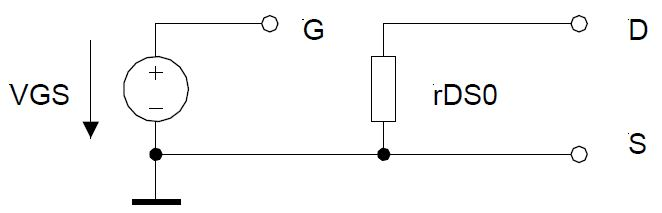
\includegraphics[height=1.5cm]{chapters/Transistoren/images/Ersatzsch_unges}&
	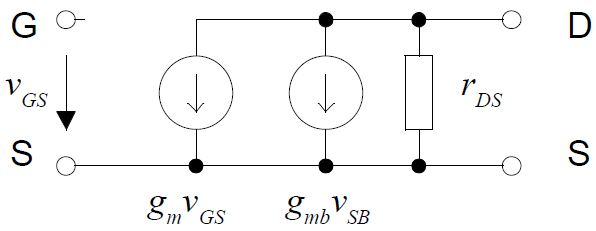
\includegraphics[height=1.6cm]{chapters/Transistoren/images/KS_ges_PI_Bulk}&
	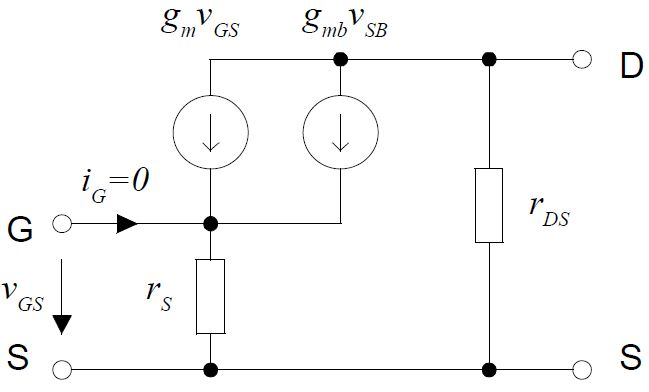
\includegraphics[height=2.2cm]{chapters/Transistoren/images/KS_ges_T_Bulk}&
	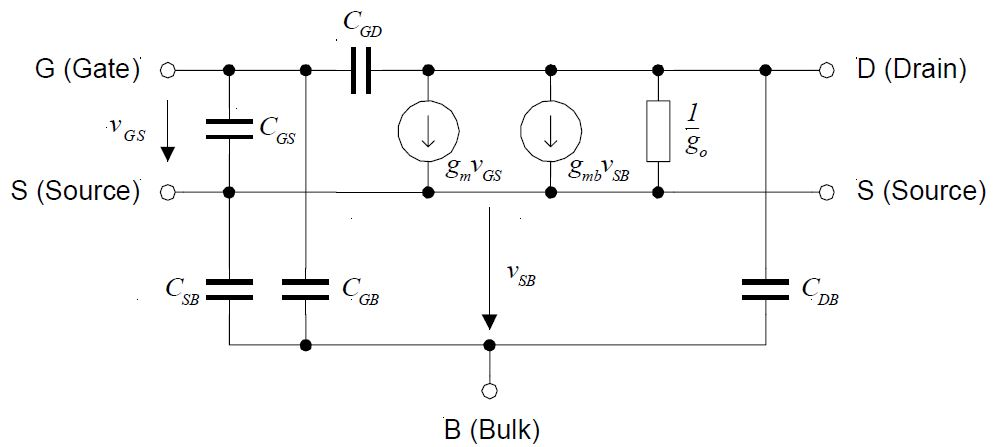
\includegraphics[height=2.2cm]{chapters/Transistoren/images/KS_HF}\\ \hline
\end{tabular}

\subsection{Kleinsignalparameter}
\begin{tabular}{|p{0.2\textwidth}|p{0.35\textwidth}|p{0.35\textwidth}|}
	\hline
	&\textbf{Transistor ungesättigt}&\textbf{Transistor gesättigt}\\ \hline
	weak inversion&Kanalwiderstand bei $V_{DS}=0$:&Kanalwiderstand:\\
	&$r_{DS0}=\frac{dV_{DS}}{dI_D}\vert_{V_{DS}=0} = \frac{\Phi_t}{I_{D0}}$ &$r_{DS}=\frac{1}{g_0}=\frac{dV_{DS}}{dI_D}=\frac{V_A+V_{DS}}{I_D}\approx\frac{V_A}{I_D}$\\
	&Kanalwiderstand bei $V_{DS} = \SI{0}{\volt} \dots V_{DS,sat}$:&\\
	&$r_{DS}=\frac{dV_{DS}}{dI_D}\approx \frac{\Phi_t}{I_D}e^{\frac{V_{DS}}{\Phi_t}}$ (ungenau, kaum benötigt)&\\ \cline{2-3}
	&$g_m$ nicht benötigt&Steilheit\\
	&&$g_m = \frac{dI_D}{V_{GS}}=\frac{I_D}{n_M\Phi_t}$\\ \hline
	strong inversion&Kanalwiderstand bei $V_{DS}=0$:&Kanalwiderstand:\\
	&$r_{DS0}=\frac{dV_{DS}}{dI_D}\vert_{V_{DS}=0}=\frac{1}{\beta(V_{GS}-V_T)\textcolor{gray}{(1+\lambda V_{DS})}}$&$r_{DS}=\frac{1}{g_0}=\frac{dV_{DS}}{dI_D}=\frac{V_A+V_{DS}}{I_D}\approx \frac{V_A}{I_D}$\\
	&Kanalwiderstand bei $V_{DS}=\SI{0}{\volt} \dots V_{DS,sat}$:&\\
	&$r_{DS}=\frac{dV_{DS}}{dI_D}=\frac{1}{\beta[(V_{GS}-V_T)-V_{DS}]\textcolor{gray}{(1+\lambda V_{DS})}}$&\\ \cline{2-3}
	&$g_m$ nicht benötigt&Steilheit (zwei Formeln)\\
	&&$g_m = \frac{dI_D}{V_{GS}}=\beta(V_{GS}-V_T)\textcolor{gray}{(1+\lambda V_{DS})}$\\
	&&$g_m = \frac{dI_D}{V_{GS}}=\sqrt{2I_D\beta\textcolor{gray}{(1+\lambda V_{DS})}}=\frac{2I_D}{V_{GS}-V_T}$\\ 
	&&$g_{mb}= \frac{dI_D}{V_{SB}}= -g_m(n_m-1)$ wobei \\ &&$n_m=1+\frac{\lambda}{2\sqrt{V_{SB}+\Phi_0}}\approx 1.5$ (bei $V_{SB}=0$)\\      \hline
\end{tabular}

\section{Grundschaltungen mit MOS-Transistoren (Kap. 6)} 

\begin{tabular}{|p{0.11\textwidth}|p{0.25\textwidth}|p{0.25\textwidth}|p{0.25\textwidth}|}
	\hline
	&\textbf{Source-Schaltung:}&\textbf{Gate-Schaltung:}&\textbf{Drain-Schaltung:} (Source-Folger)\\
	\textbf{Schema}&
	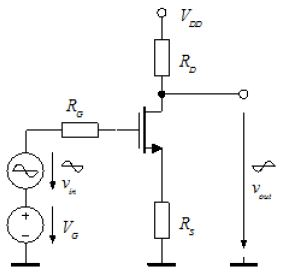
\includegraphics[height=3cm]{chapters/Transistoren/images/GschSource}&
	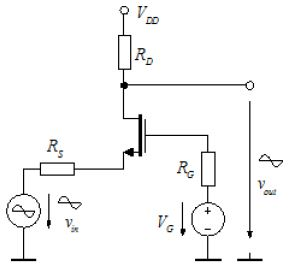
\includegraphics[height=3cm]{chapters/Transistoren/images/GschGate}&
	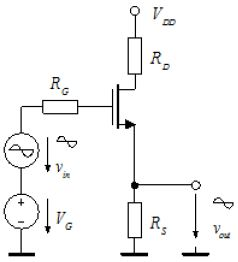
\includegraphics[height=3cm]{chapters/Transistoren/images/GschDrain}\\ \hline
	\textbf{Art}&Invertierender Verstärker&Nichtinvertierender Verstärker&Nichtinvertierender Verstärker\\ \hline
	\textbf{Anwendung}&Verstärkung tiefe bis mittlere Frequenzen&Verstärker hohe Frequenzen (HF-Verstärker)&Spannungsfolger / Impedanzwandler / Leistungstreiber\\ \hline
	\textbf{Eingang}&Gate&Source&Gate\\ \hline
	\textbf{Ausgang}&Drain&Drain&Source\\ \hline
	\textbf{$R_{in}$ / $R_{out}$}&gross/gross&klein/gross&gross/klein\\ \hline
	\textbf{Verstärkung}&\textbf{Bei $1/g_m$,$R_D<<1/g_0$:}&Bei $1/g_m$,$R_D<<1/g_0$:&Bei $R_S$,$R_D<<1/g_0$:\\
	&$a\approx -\frac{R_D}{R_S+\frac{1}{g_m}}$&$a\approx \frac{R_D}{R_S+\frac{1}{g_m}}$&$a\approx \frac{R_S}{R_S+\frac{1}{g_m}}$\\
	&Bei $R_S = 0$: &Bei $R_S = 0$: &Idealer Source-Folger: $a\approx 1$\\
	&$a\approx -g_m(R_D||r_{DS})$&$a\approx g_m(R_D||r_{DS})(1+\frac{g_0}{g_m})$&($1/g_m<<R_S<<1/g_0$)\\ \hline
	\multicolumn{4}{|l|}{$g_m=\frac{1}{r_S}$ \hspace{5mm} $g_0=\frac{1}{r_{DS}}=\frac{I_D}{V_A+V_{DS}}\approx\frac{I_D}{V_A}$ (Näherung für $V_A >> V_{DS}$) \hspace{5mm} $V_A = a_A \cdot L$ ($V_A = \SI{5}{\volt}\dots \SI{100}{\volt}$,Kanallängenabh.)}\\ \hline
\end{tabular} \\ [1ex]
\textbf{Innenwiderstände}\\
\begin{tabular}{|p{0.3\textwidth}|p{0.3\textwidth}|p{0.3\textwidth}|}
	\hline
	\textbf{Drain}&\textbf{Gate}&\textbf{Source}\\
	\hline
	Näherung für $1/g_0>>R_s$&$r_{iG}\rightarrow \infty$&Näherung für $1/g_0>>R_D$\\
	$r_{iD}\approx r_{DS}(1+\frac{R_S}{r_s})=\frac{1}{g_0}(1+g_mR_s)$&&$r_{iS}\approx r_s||r_{DS}=\frac{1}{g_m+g_0}$ \\
	Näherung für $R_s=0$&&Näherung für $g_m$, $1/R_D>>R_D$\\
	$r_{iD}\approx r_{DS}=\frac{1}{g_0}$&&$r_{iS}\approx r_S=\frac{1}{g_m}$\\
	\hline
\end{tabular}
% !TeX spellcheck = de_CH_frami

\section{MOS-Diode (Kap. 7)}
Um eine MOS-Diode aus einem MOS-Transistor zu erhalten, werden die Anschlüsse von Gate und Drain verbunden.\\
\begin{tabular}{|p{0.11\textwidth}|p{0.14\textwidth}|p{0.16\textwidth}|p{0.145\textwidth}|p{0.125\textwidth}|p{0.2\textwidth}|}
	\hline
	\multicolumn{2}{|c|}{\textbf{Reale Diode:}}&\multicolumn{4}{c|}{\textbf{MOS-Diode:}}\\ \hline
	Symbol&Kennlinie&N-MOS-Diode&P-MOS-Diode&Kennlinie&KS-Ersatzschaltung\\
	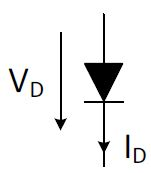
\includegraphics[height=2.6cm]{chapters/Diode/images/realeDiode}&
	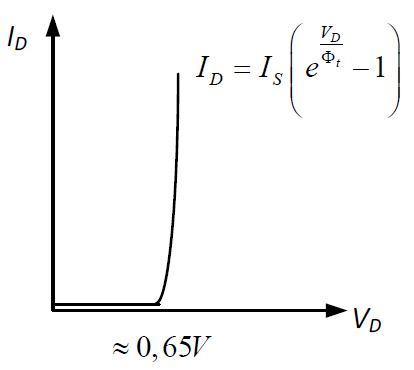
\includegraphics[height=2.6cm]{chapters/Diode/images/KennlinieRealeDiode}&
	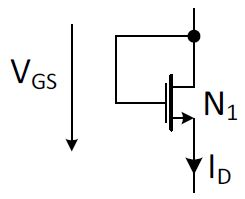
\includegraphics[height=2.6cm]{chapters/Diode/images/NMOS-Diode}&
	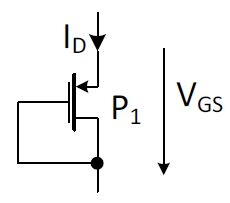
\includegraphics[height=2.6cm]{chapters/Diode/images/PMOS-Diode}&
	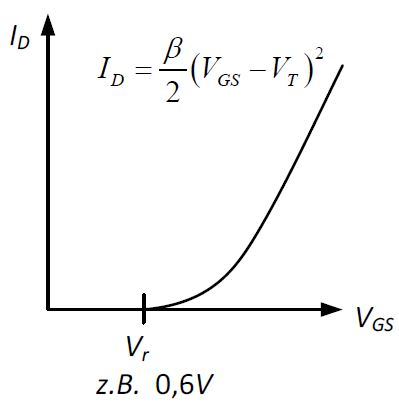
\includegraphics[height=2.6cm]{chapters/Diode/images/KennlinieDiode}&
	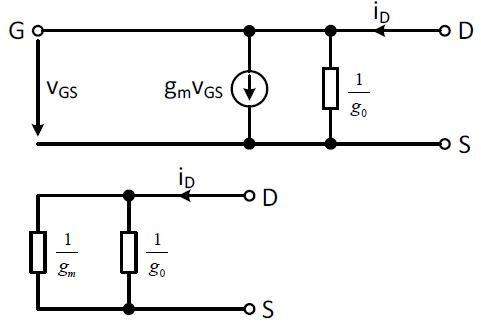
\includegraphics[height=2.6cm]{chapters/Diode/images/KS_Diode}\\ \hline
\end{tabular}\\[1ex]
\begin{tabular}{|l|l|}
	\hline
	Arbeitspunktstrom einer MOS-Diode mit Widerstandslast $R_D$&$I_D=\frac{\beta}{2}(V_{GS}-V_T)^2\textcolor{gray}{(1+\lambda V_{DS})} = \frac{V^+-V_{GS}}{R_D}$\\ \hline
	$V_{DS}$ einer MOS-Diode bei gegebenem Strom&$V_{DS}=V_T + \sqrt{\frac{2I_D}{\beta \textcolor{gray}{(1+\lambda V_{DS})}}}\approx V_T + \sqrt{\frac{2I_D}{\beta}}$\\ \hline
	Innenwiderstand der MOS-Diode&$r_{MD}=\frac{v_{GS}}{i_D}=\frac{1}{g_m+g_0}\approx\frac{1}{g_m}$\\ \hline
	Im quadratischen Bereich gilt:&$g_m=\beta(V_{GS}-V_T)=\sqrt{2\beta I_D}$\\ \hline
\end{tabular}\\ [1ex]
Bei der leitenden MOS-Diode ist der Transistor immer gesättigt, weil $V_{DS}>V_{DS,sat} = (V_{GS}-V_T)$ jederzeit erfüllt ist.
\textbf{MOS-Dioden als Spannungsteiler}\\
\begin{tabular}{|p{0.15\textwidth}|p{0.3\textwidth}|p{0.15\textwidth}|p{0.15\textwidth}|}
	\hline
	\textbf{Mit Bodyeffekt}&\textbf{Ohne Bodyeffekt}&\multicolumn{2}{l|}{\textbf{Mehrfach Spannungsteiler}}\\ \hline
	$V_{SB1}=0$, $V_{SB2}=V_{GS1}$ daher Body-Effekt und $V_{T2} > V_{T1}$&$V_{SB1}=0$,$V_{SB2}=0$ daher kein Body-Effekt. Es gelten die Nominalwerte für $V_{T2}$, $V_{T1}$&Lokales Substrat, $V_{Ti}$ für alle gleich $\rightarrow$ gleiche Teilspannungen&Gemeinsames Substrat, unterschiedliche $V_{Ti}$ $\rightarrow$ unterschiedliche Teilspannungen\\
	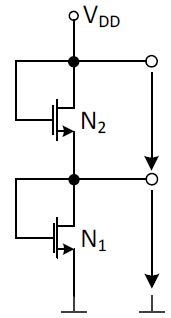
\includegraphics[height=2.6cm]{chapters/Diode/images/SpgT_N_Bodyeffekt}&
	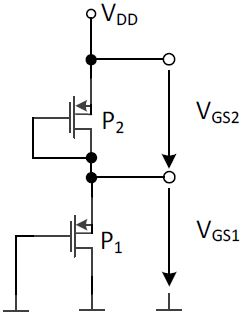
\includegraphics[height=2.6cm]{chapters/Diode/images/SpgT_P_body}
	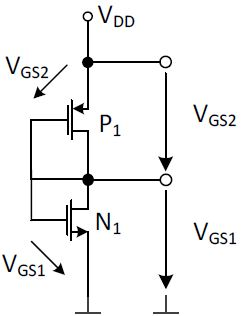
\includegraphics[height=2.6cm]{chapters/Diode/images/SpgT_PN}&
	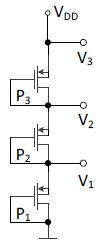
\includegraphics[height=2.6cm]{chapters/Diode/images/SpgT_P3}&
	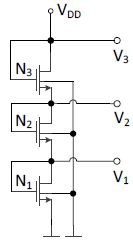
\includegraphics[height=2.6cm]{chapters/Diode/images/SpgT_N3}\\
	\hline	
\end{tabular}
% !TeX spellcheck = de_CH_frami

\section{MOS-Transistor als Stromquelle (Kap. 8)}
Die Drain-Source-Strecke des MOS-Transistors stellt im Sättigungsbetrieb eine gesteuerte Stromquelle dar, deren Ausgangswiderstand (Innenwiderstand am Drain) relativ hoch ist.\\
\begin{minipage}[c]{0.45\textwidth}
	\subsection{Strom einer MOS Stromquelle}
	$I_D=\frac{\beta}{2}(V_{GS}-V_T)^2\textcolor{gray}{(1+\lambda V_{DS})} \approx \frac{\beta}{2}(V_{GS}-V_T)^2$\\
\end{minipage}
\begin{minipage}[c]{0.55\textwidth}
	\subsection{Sättigungsspannung}
	\textbf{Bei starker Inversion} $V_{DS} \geq V_{DS,sat}=V_{GS}-V_T=\sqrt{\frac{2I_D}{\beta}}$\\
	\textbf{Bei schwacher Inversion} $V_{DS} \geq V_{DS,sat}\approx 5\Phi_t \approx \SI{130}{\milli\volt}$
\end{minipage}\\
\begin{tabular}{|p{0.3025\textwidth}|p{0.3025\textwidth}|p{0.3025\textwidth}|}
	\hline
	\textbf{einfache Stromquelle mit und ohne Source-Widerstand}&\textbf{Stromquelle mit Kaskode}&\textbf{Stromquelle mit geregelter Kaskode}\\
	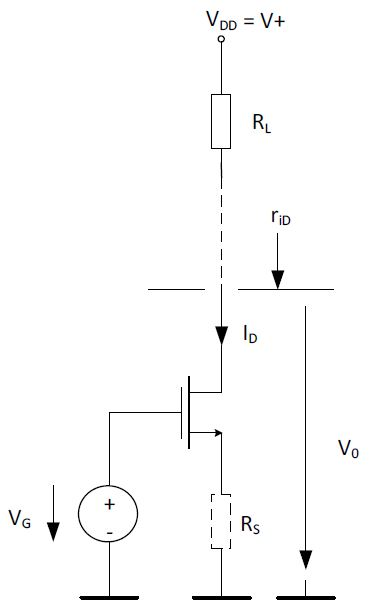
\includegraphics[height=4.8cm]{chapters/Stromquelle/images/einfacheStromquelle}&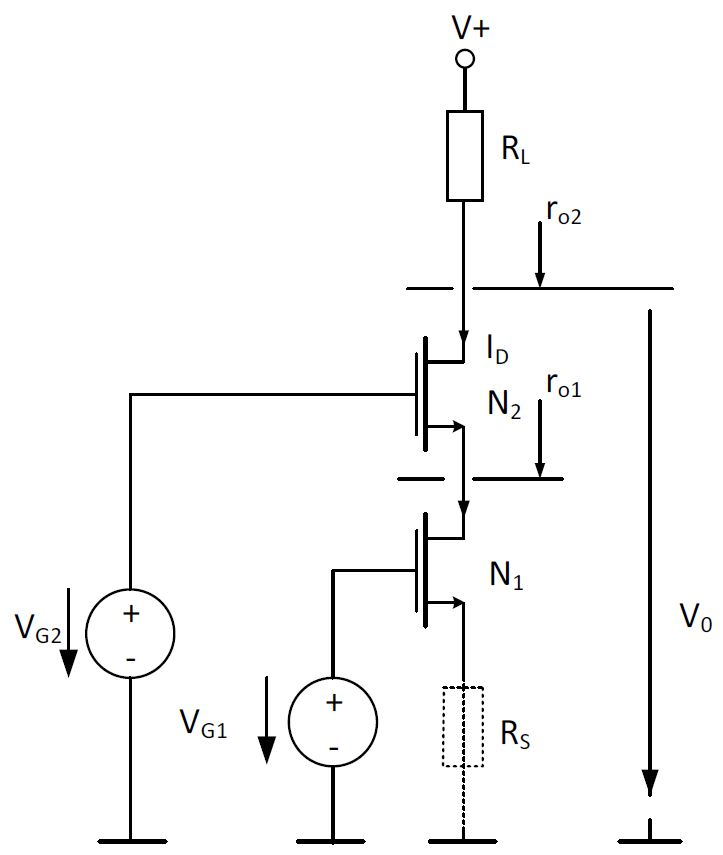
\includegraphics[height=4.8cm]{chapters/Stromquelle/images/Kaskode}&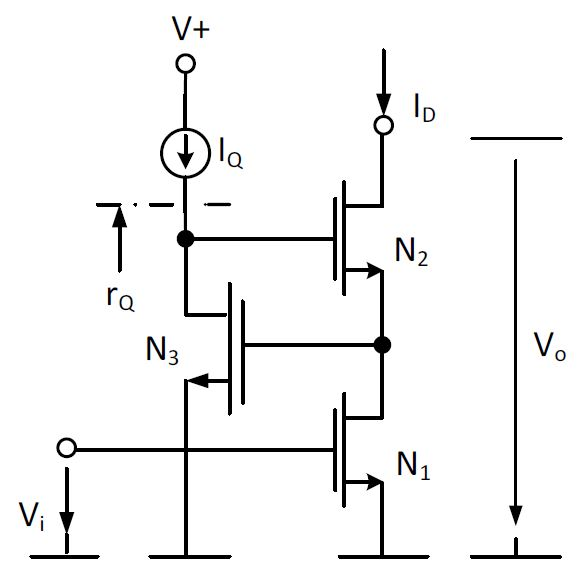
\includegraphics[height=4.8cm]{chapters/Stromquelle/images/geregelteKaskode}\\ \hline
\end{tabular} \\
\begin{longtable}{|l|l|l|}
	\hline
	\textbf{Konfiguration}&\textbf{Ausgangswiderstand $r_0$}&\textbf{min. Ausgangsspannung $V_{0,min}$}\\ \hline
	\endhead
	Einfache Quelle &$r_{out}=r_{iD}=r_{DS}=\frac{1}{g_0}=$&$V_0 > V_{0,min}=V_{DS,sat}$\\
	mit 1 Transistor&$\frac{V_A+V_{DS}}{I_D}\approx \frac{V_A}{I_D}$&\\ \hline
	Stromquelle mit &$r_{iD}=r_{DS}(1+\frac{R_S}{r_S}+\frac{R_S}{r_{DS}})=$&$V_0 > V_{0,min} = R_S I_D + V_{DS,sat}$\\
	Source-Widerstand&$\frac{1}{g_0}\left( 1+g_mR_S\right) + R_S$&\\ \hline
	Stromquelle mit Kaskode&$r_{out}=r_{o2}\approx \frac{r^2_{DS}}{r_{S2}}=$&$V_{0,min}=V_{G2}-V_{GS2}+V_{DS2,sat}$\\
	&$\left( \frac{r_{DS}}{r_S} \right) r_{DS}=\mu\cdot r_{DS}=\frac{1}{g_{o1}}\cdot\frac{g_{m2}}{g_{o2}}$ &$V_{0,min}=V_{DS1,sat}+V_{DS2,sat}$\\
	&&(mit $V_{G2}=V_{DS1,sat}+G_{GS2}$)\\ \hline
	Stromquelle mit geregelter Kaskode&$r_{out}\approx r_{DS1}\cdot\frac{r_{DS2}}{r_{S2}}\cdot\frac{r_{DS3}}{r_{S3}}=\frac{1}{g_{o1}}\cdot\frac{g_{m2}}{g_{o2}}\cdot\frac{g_{m3}}{g_{o3}}$&$V_{0,min}=2V_{DS,sat}$ \\ \hline
\end{longtable}
% !TeX spellcheck = de_CH_frami

\section{MOS-Stromspiegel (Kap. 9)}

\begin{minipage}[t]{0.25\textwidth}
	\textbf{Stromspiegelverhältnis}\\
	$n_m=\frac{I_{out}}{I_{in}}=\frac{(\frac{W}{L})_{2}}{(\frac{W}{L})_{1}}$
\end{minipage}
\begin{minipage}[t]{0.35\textwidth}
	\textbf{Berechnung Ausgangsstrom}\\
	$I_{out}=I_{in}\cdot\frac{(\frac{W}{L})_{2}}{(\frac{W}{L})_{1}}$ (allgemein)\\
	$I_{out}=I_{in}\cdot \frac{W_{T2}}{W_{T1}}$ (wenn $L_{T2}=L_{T1}$)
\end{minipage}
\begin{minipage}[t]{0.35\textwidth}
	\textbf{Impedanzen}\\
	Eingangsimpedanz (ideal): $r_{in}=0\Omega$\\
	Ausgangsimpedanz (ideal): $r_{out}=\infty\Omega$
\end{minipage}\\
\begin{tabular}{|p{0.4\textwidth}|p{0.525\textwidth}|}
	\hline
	\textbf{Widlar-Stromspiegel}&\textbf{Wilson-Stromspiegel}\\
	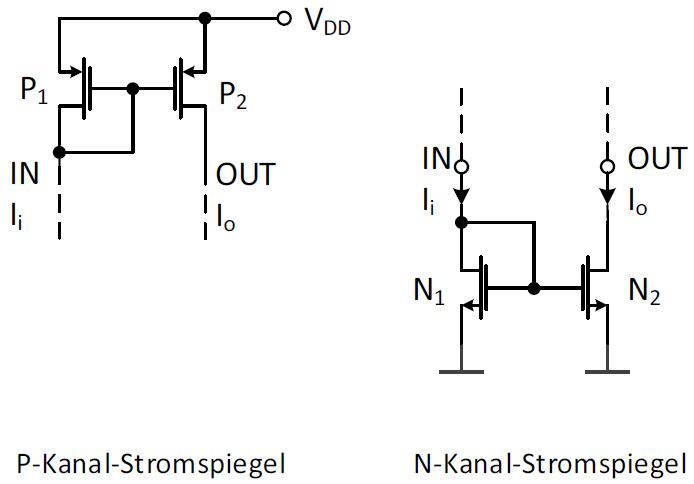
\includegraphics[height=5cm]{chapters/Stromspiegel/images/Widlar}&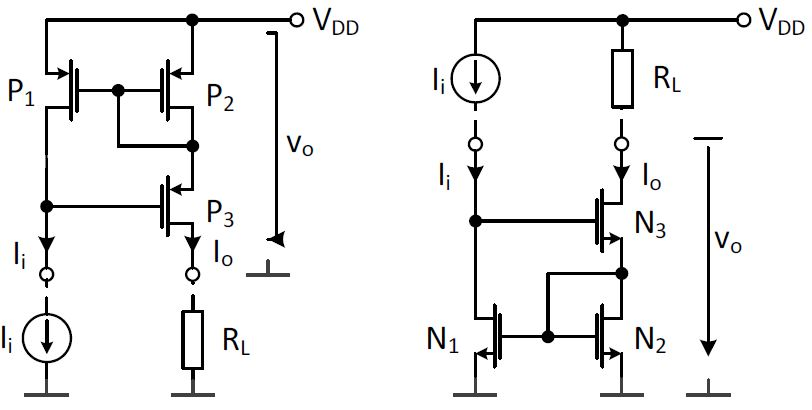
\includegraphics[height=5cm]{chapters/Stromspiegel/images/Wilson}\\ \hline
\end{tabular}\\
\begin{tabular}{|p{0.25\textwidth}|p{0.25\textwidth}|p{0.402\textwidth}|}
	\hline
	\textbf{verbesserter Wilson-Stromspiegel}&\textbf{Kaskode}&\textbf{geregelte Kaskode}\\
	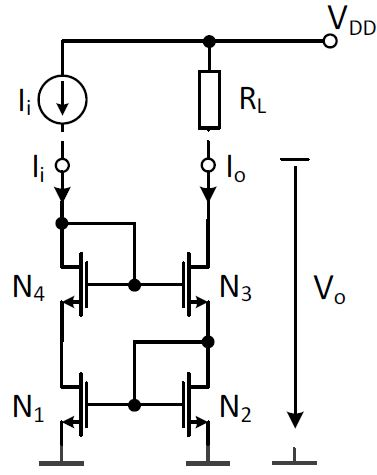
\includegraphics[height=5cm]{chapters/Stromspiegel/images/verbesserterWilson}&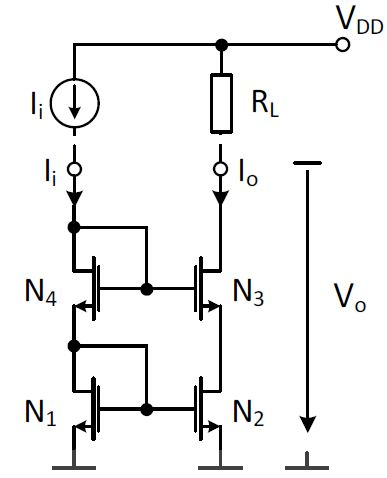
\includegraphics[height=5cm]{chapters/Stromspiegel/images/Kaskode}&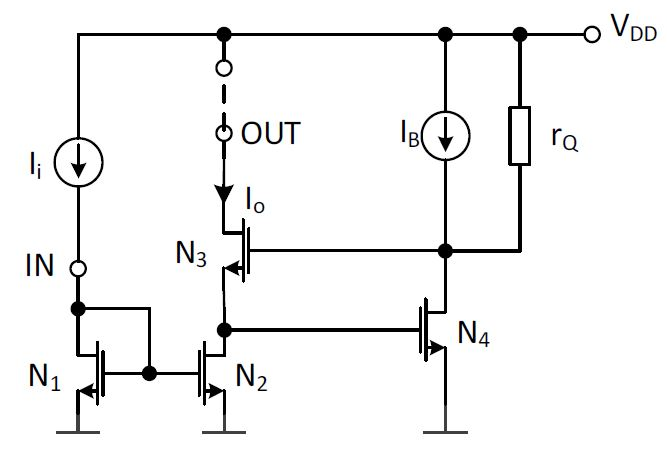
\includegraphics[height=5cm]{chapters/Stromspiegel/images/geregelteKaskode}\\ \hline
\end{tabular}\\[2ex]
\begin{tabular}{|l|l|l|l|l|}
	\hline
	\textbf{Stromspiegeltyp}&\textbf{Genauigkeit}&\textbf{$r_{out}$}&\textbf{$V_I$}&\textbf{$V_{O,min}$}\\ \hline
	Widlar-Stromspiegel&+&$=\frac{1}{g_0}$&$\approx V_T + \sqrt{\frac{2I_I}{\beta}}$&$\approx \sqrt{\frac{2I_0}{\beta}}$\\ \hline
	Wilson-Stromspiegel&+&$\approx \frac{1}{g_0}(2+\frac{g_m}{g_0})$&$\approx 2V_T+2\sqrt{\frac{2I_I}{\beta}}$&$\approx V_T+2\sqrt{\frac{2I_0}{\beta}}$\\ \hline
	Verbesserter Wilson&++&$\approx \frac{1}{g_0}(2+\frac{g_m}{g_0})$&$\approx 2V_T+2\sqrt{\frac{2I_I}{\beta}}$&$\approx V_T+2\sqrt{\frac{2I_0}{\beta}}$\\ \hline
	Kaskode-Stromspiegel&++&$\approx \frac{1}{g_0}(2+\frac{g_m}{g_0})$&$\approx 2V_T+2\sqrt{\frac{2I_I}{\beta}}$&$\approx V_T+2\sqrt{\frac{2I_0}{\beta}}$\\ \hline
	geregelte Kaskode&++&$\approx\frac{1}{g_0}(\frac{g_m}{g_0})^2$&$\approx V_T+\sqrt{\frac{2I_I}{\beta}}$&$\approx 2\sqrt{\frac{2I_0}{\beta}}$\\ \hline
\end{tabular}
% !TeX spellcheck = de_CH_frami
\newpage
\section{Einstufige MOS-Verstärker (Kap. 10)}
Grosssignal-Analyse (Arbeitspunktberechnung)\\
Kleinsignal-Analyse (Signalberechnung)\\
\textbf{Tipp:} Jede Gate-Drain Strecke invertiert das Vorzeichen der Kleinsignalübertragung.\\
\begin{tabular}{|p{0.16\textwidth}p{0.44\textwidth}|p{0.3\textwidth}|}
	\hline
	\textbf{Verstärker mit Widerstandslast}&\textbf{Kleinsignal Ersatzschaltung}&\textbf{Verstärker mit MOS-Dioden-Last}\\
	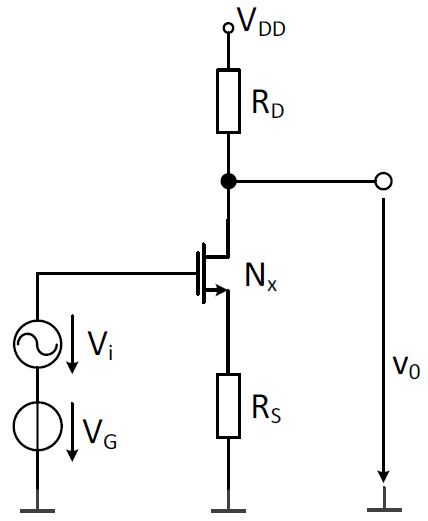
\includegraphics[height=3.5cm]{chapters/Verstaerker/images/AmpWiderstand}&
	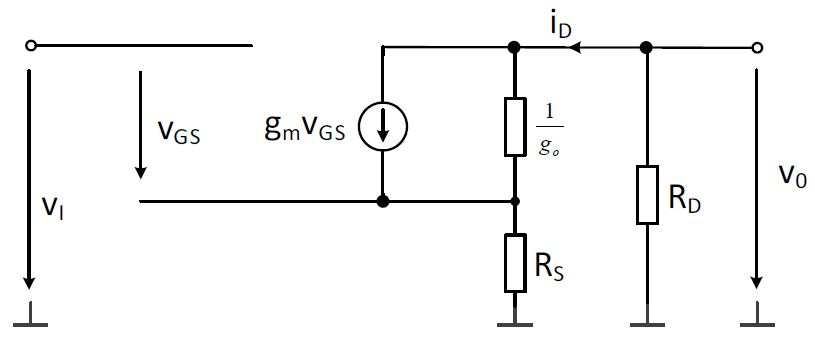
\includegraphics[height=3.5cm]{chapters/Verstaerker/images/AmpWiderstandKS}&
	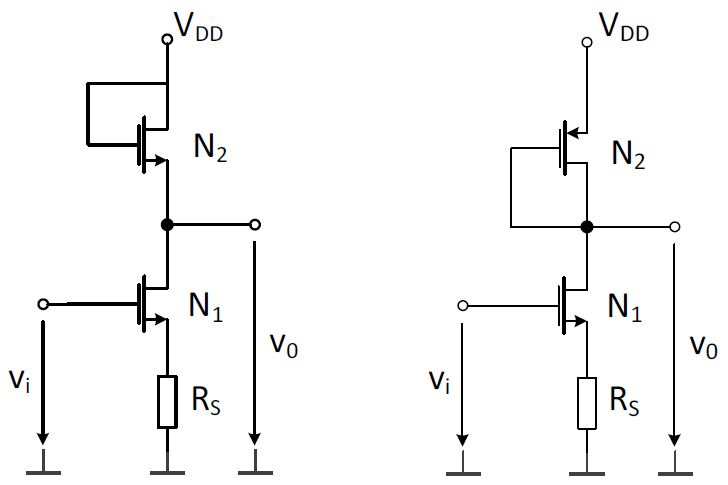
\includegraphics[height=3.5cm]{chapters/Verstaerker/images/AmpDiode}\\ 
\end{tabular}\\
\begin{tabular}{|p{0.18\textwidth}p{0.2\textwidth}|p{0.25\textwidth}|p{0.245\textwidth}|}
	\hline
	\textbf{Verstärker mit Stromquellenlast}&\textbf{Realisierung}&\textbf{Verstärker mit parallelem Eingang (Push-Pull)}&\textbf{Verstärker mit Stromumlenkung}\\
	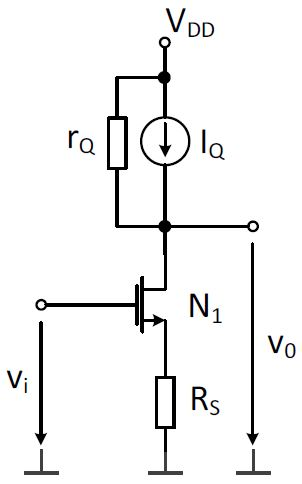
\includegraphics[height=3.5cm]{chapters/Verstaerker/images/AmpStromquelle}&
	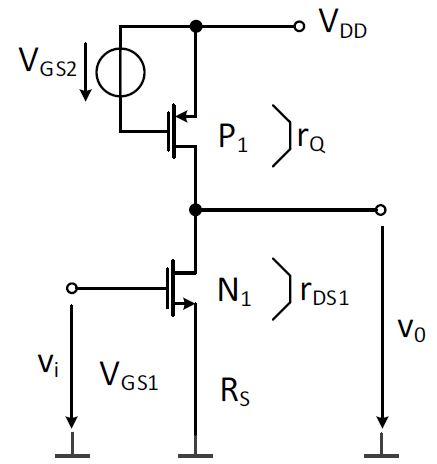
\includegraphics[height=3.5cm]{chapters/Verstaerker/images/AmpStromquelleReal}&
	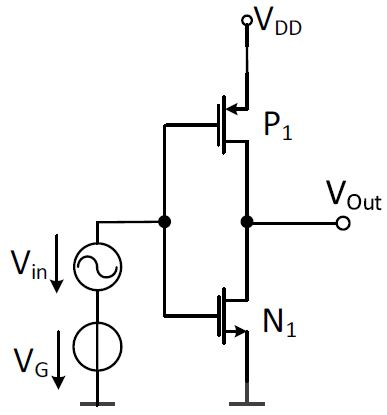
\includegraphics[height=3.5cm]{chapters/Verstaerker/images/AmpPushPull}&
	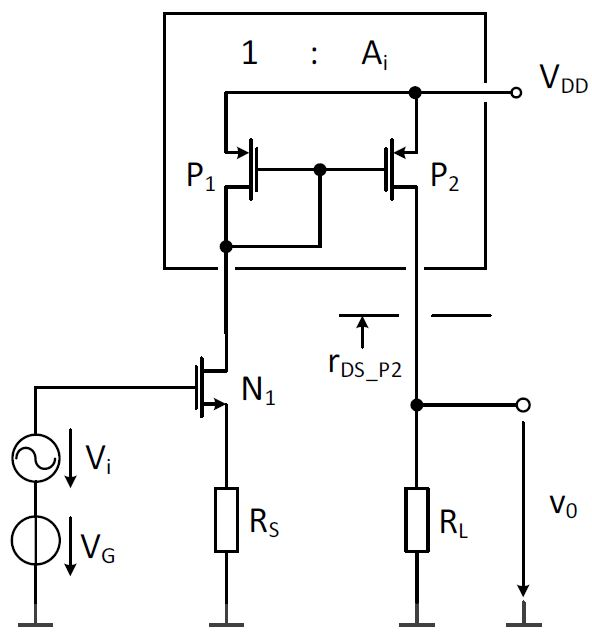
\includegraphics[height=3.5cm]{chapters/Verstaerker/images/AmpStromumlenkungR}
\end{tabular}\\
\begin{tabular}{|p{0.3\textwidth}|p{0.3\textwidth}|p{0.3\textwidth}|}
	\hline
	\textbf{Kaskode mit Widerstandslast}&\textbf{Kaskode mit Stromquellenlast}&\textbf{Gefaltete Kaskode}\\
	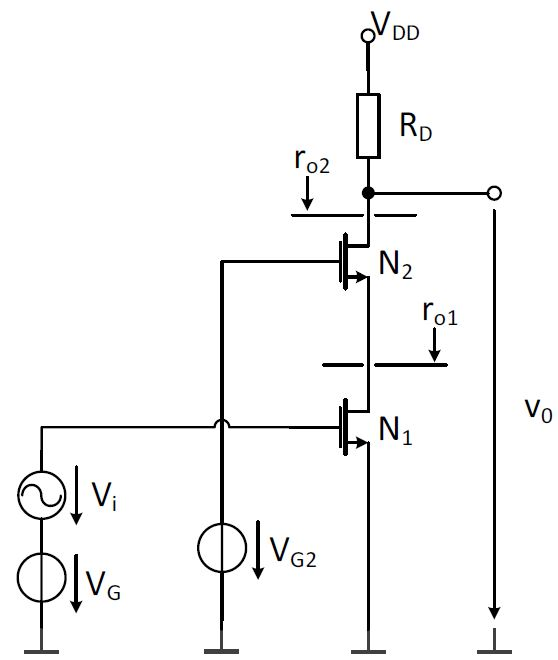
\includegraphics[height=3.5cm]{chapters/Verstaerker/images/AmpKaskodeR}&
	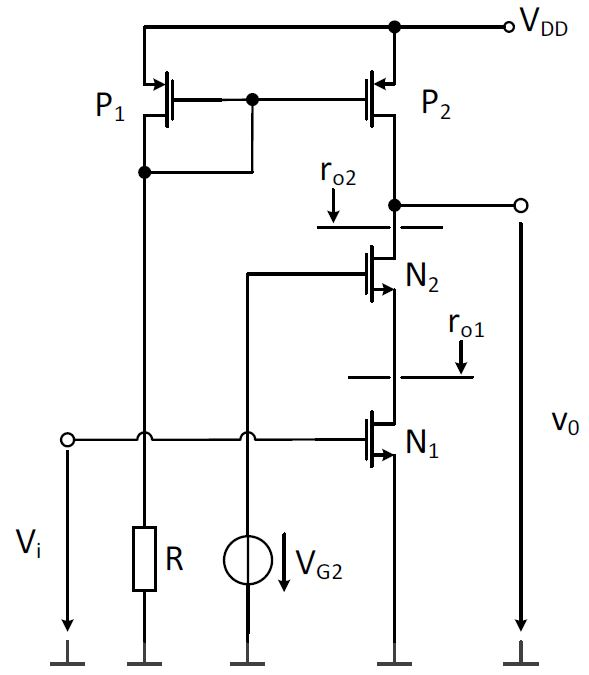
\includegraphics[height=3.5cm]{chapters/Verstaerker/images/AmpKaskodeIq}&
	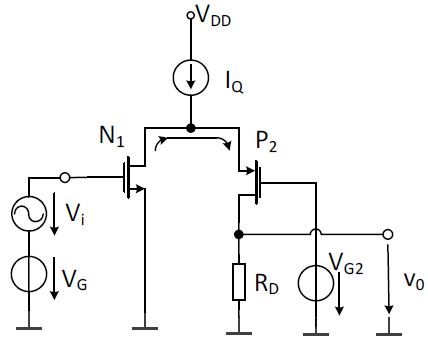
\includegraphics[height=3.5cm]{chapters/Verstaerker/images/AmpFoldedKaskode}\\ \hline
\end{tabular}\\
\begin{tabular}{|l|l|}
	\hline
	Verstärker mit Widerstandslast&$a=-\frac{g_m}{\frac{1}{R_D}+g_0}$\\
	&$r_{out}=r_{iD}=\frac{1}{g_0}(1+g_mR_S)+R_S$\\ \hline
	Verstärker mit MOS-Dioden-Last&$a=-\frac{\frac{1}{g_{m2}}}{R_S+\frac{1}{g_{m1}}}\textcolor{gray}{=-\frac{g_{m1}}{g_{m2}}=-\sqrt{\frac{\beta_1}{\beta_2}}}$ \textcolor{gray}{(wenn $R_S = 0$)}\\ \hline
	Verstärkung mit Stromquellenlast&$a=-\frac{R_D}{R_S+\frac{1}{g_m}+(R_D+R_S)\frac{g_o}{g_m}} \textcolor{gray}{=-\frac{g_{m1}}{\frac{1}{r_Q}+g_{o1}}}$\\ \hline
	Verstärker mit parallelem Eingang (Push-Pull-Stufe)&$a=-\frac{g_{m\_N1}+g_{m\_P1}}{g_{o\_N1}+g_{o\_P1}}= -(g_{m\_N1}+g_{m\_P1})\cdot (r_{DS\_N1}||r_{DS\_P1})$\\ \hline
	Verstärker mit Stromumlenkung&$a\approx a_i\frac{R_L||r_{DS3}}{R_S+r_{S1}}$\\ \hline
	Kaskode mit Widerstandslast&$a\approx -g_{m1}R_D$\\ \hline
	Kaskode mit Stromquellenlast&$a \approx -\frac{g_{m1}}{g_{o3}}$ \\ \hline
\end{tabular}
%% !TeX spellcheck = de_CH_frami

\section{Frequenzverhalten von MOS-Verst�rkern (Kap. 11)}
\includegraphics[width=1\linewidth]{chapters/Frequenzverhalten/images/parasit�re_kapazit�ten}

% !TeX spellcheck = de_CH_frami
\section{MOS Operationsverstärker (Kap. 12)}
\begin{minipage}[c]{0.5\textwidth}
	\textbf{OTA:} Hohe Eingangsimpedanz, hohe Ausgangsimpedanz. Verhalten einer spannungsgesteuerten Stromquelle.
\end{minipage}
\begin{minipage}[c]{0.5\textwidth}
	\textbf{OpAmp:} Hohe Eingangsimpedanz, tiefe Ausgangsimpedanz. Verhalten einer spannungsgesteuerten Spannungsquelle.
\end{minipage}

\subsection{Struktur}
\begin{minipage}[c]{0.3\textwidth}
	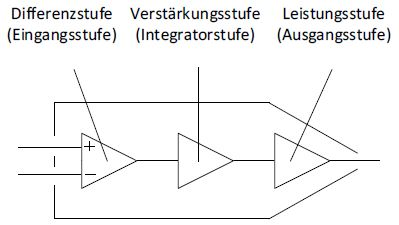
\includegraphics[width=1\linewidth]{chapters/OpAmp/images/Blockstruktur}
\end{minipage}
\begin{minipage}[c]{0.7\textwidth}
	\textbf{Differenzstufe} bildet die Differenz der beiden Eingangssignale und verstärkt sie mit dem Differenzverstärkungsfaktor.\\
	\textbf{Verstärkungsstufe} erhöht die Gesamtverstärkung. Bestimmt meist die Gesamtbandbreite des Operationsverstärkers.\\
	\textbf{Leistungsstufe} wandelt die Impedanz. Verstärkung ist selten grösser als eins. Verkleinert den Ausgangswiderstand und stellt genügend Ausgangsstrom zur Verfügung.\\[1ex]
	\textbf{Hinweis:} In seltenen Fällen sind erste und zweite oder auch zweite und dritte Stufe differenziell gekoppelt.
\end{minipage}

\subsection{Differenzstufe}
Eigenschaften der Differenzstufe bei starker Inversion:\\
\begin{tabular}{ll}
	$V_d = \pm \frac{1}{2}\sqrt{\frac{I_Q}{\beta}}$& Linearität der Diff-Stufe gut. An der Linearitätsgrenzen fliesst $I_D = \SI{0.74}{I_Q}$ bzw. $I_D = \SI{0.26}{I_Q}$.\\
	$V_d = \pm\sqrt{\frac{I_Q}{\beta}}$& In einem der Zweige fliesst $I_D = \SI{0.93}{I_Q}$, im anderen $I_D = \SI{0.07}{I_Q}$.\\
	$V_d = \pm\sqrt{2}\sqrt{\frac{I_Q}{\beta}}$& Der gesamte $I_Q$ fliesst in einem der beiden Zweigen.
\end{tabular}

\subsection{Slew-Rate}
\begin{compactenum}
	\item SR jeder einzelnen Verstärkerstufe untersuchen
	\item SR auf den Ausgang beziehen ($\cdot a$)
	\item Verstärkerstufe mit kleinster SR ist dominant.
\end{compactenum}
	\begin{tabular}{ll}
		Definition Slew-Rate&$SR=\frac{dv_o}{dt}=\frac{I_{out}}{C_L}$ [\SI{}{\volt/\micro\second}]\\
		Differenzstufe (einstufig)& $SR_r = |SR_f|=\frac{I_Q}{C_L}$\\
		Mit Verstärkung nach SR-dominanter Stufe&$|SR|=\frac{dv_{CL}}{dt}\cdot a= \frac{I_Q}{C_L}\cdot a$
	\end{tabular}\\[1ex]
	Designregel für grosse SR: $I_Q$ gross, $C_L$ klein.

\subsection{Wichtige Kenndaten/Formeln}
\begin{tabular}{p{0.3\textwidth}p{0.6\textwidth}}
	Transkonduktanz Differenzstufe & Ohne Stromspiegel $g_{md}=\frac{\delta I_{out}}{\delta V_d}=\frac{i_{out}}{v_d}=-\frac{g_m}{2}$ \\
	& Mit Stromspiegel $g_{md}=\frac{\delta I_{out}}{\delta V_d}=\frac{i_{out}}{v_d}=-g_m$ \\
	Verstärker Differenzstufe&Bei Widerstandslast $i_{out}=-\frac{g_mv_d}{2}$; $a\approx \frac{g_mr_{out}}{2}$\\
	&Bei Stromspiegellast $i_{out}=-g_mv_d$; $a\approx g_m\cdot r_{out}$\\
	Grenzwert bei starker Inversion& $a=V_A \sqrt{\frac{\beta}{I_Q}}$ (Bedingung: ${a_E}_N = {a_E}_P$)\\
	Grenzwert bei schwacher Inversion& $a=\frac{V_A}{2n_M \Phi_t}$\\
	Gain-Bandwith-Product& $GBP=|a|\cdot f_{P1}=-\frac{g_m}{2\pi C_L}$\\
	Input Common Mode Range&$V_{inp,max}=(V_{DD}-V_{SS})-V_{GS,P1}-V_{DSsat,N1}+V_{GS,N1}$\\
	&$V_{inp,min}=V_{SS}+V_{DSsat,N5}+V_{GS,N1}$\\[2ex]
	&Wenn $V_{DSsat}\approx \sqrt{\frac{2I_D}{\beta}}$ dann gilt:\\
	&$V_{inp,max}=(V_{DD}-V_{SS})-V_{T,P1}-\sqrt{\frac{I_{SS}}{\beta P_1}}+V_{T,N1}$\\
	&$V_{inp,min}=V_{SS}+\sqrt{\frac{2I_{SS}}{\beta N_5}}+V_{T,N}+\sqrt{\frac{I_{SS}}{\beta N_1}}$\\
	Common mode rejection ratio&$v_{DM}=v_{in1}-v_{in2}$ differential mode\\
	&$v_{CM}=\frac{v_{in1}+v_{in2}}{2}$ common mode\\
	&$a_{DM}=\left.\frac{v_O}{V_{DM}}\right|_{v_{CM}=0}$ (ideal $a_{DM}=\infty$) Gegentaktverstärkung\\
	&$a_{CM}=\left.\frac{v_O}{V_{CM}}\right|_{v_{DM}=0}$ (ideal $a_{CM}=0$) Gleichtaktverstärkung\\
	&$CMRR=|\frac{a_{DM}}{a_{CM}}|=\frac{r_q}{r_s}=\frac{g_m}{g_{0b}}$ mit $r_q$: Innenwiderstand von $I_q$, Gleichtaktunterdrückung\\
	Power supply rejection ratio& $a_{ps}=\left.\frac{\delta V_O}{\delta V_{DD}}\right|_{V_I=konst}
	=\left.\frac{v_O}{v_{DD}}\right|_{v_I=0}$ \\
	&$PSRR_+=|\frac{a_{DM}}{a_{PS+}}|$\\
	&$PSRR_-=|\frac{a_{DM}}{a_{PS-}}|$\\
	Offset-Designregeln& \textbf{Random Offset}\\
	&Matching von Parametern der Transistoren: Layout für gutes Matching $\rightarrow$ Common Centroid, höheres $V_{GS}-V_T$ für Stromspiegel, grosses W/L für Eingangstransistoren\\
	&\textbf{Systematic Offset}\\
	&Symmetrie der Differenzstufe, gleiche $V_{DS}$ und $L$ der zu einem Stromspiegel gehörenden Transistoren, gleiche Stromdichten $\frac{I_D}{W/L}$ in Stromspiegeltransistoren\\
	& \textbf{}
\end{tabular}
% !TeX spellcheck = de_CH_frami
\section{Stabilität von MOS Operationsverstärker (Kap. 13)}
Loop-Gain $T(s)$: $T(s) = A(s)\cdot F(s)$\\
\begin{tabular}{|l|l|}
	\hline
	Phasenmarge bei& Verhalten des Verstärkers\\
	$f_{krit}$ ($a_L = 1$)& (System mit zwei weit auseinanderliegenden Polen)\\ \hline
	$\varphi_M \leq \SI{0}{\degree}$& Gegenkoppelter Verstärker schwingt selbständig\\ \hline
	$\varphi_M > \SI{0}{\degree}$& Gedämpftes Überschwingen der Sprungantwort\\ \hline
	$\varphi_M = \SI{65}{\degree}$& Peaking verschwindet. Einziger Überschwinger mit \SI{4.7}{\percent} Sprunghöhe\\ \hline
	$\varphi_M \geq \SI{75}{\degree}$& Kein Überschwingen\\ \hline
\end{tabular}\\[2ex]
\begin{tabular}{ll}
	Stabilitätskriterien&$\phi = \SI{180}{\degree} => |A(s)\cdot F(s)| < 1$\\
	&$|A(s)\cdot F(s)| = 1 => \SI{180}{\degree}-\Phi > 0; \varphi_M > \SI{0}{\degree}$\\
	Phasenmarge&$\varphi_M = \SI{180}{\degree}-\Phi = \SI{90}{\degree}-arctan(\frac{GBP}{f_{P2}})$\\
	Designregel&Wähle 2. Pol ($f_{nd}$) bei ca. $3\cdot GBP$\\
	&Dies ergibt eine Phasenmarge von \SI{72}{\degree} und somit kaum Überschwingen
\end{tabular}\\[2ex]
\begin{minipage}[c]{0.45\textwidth}
	Jeder Knoten $N$ bildet einen Pol bei der Frequenz $f_N$, der sich wie folgt berechnet:
	$f_N=\frac{1}{2\pi\cdot R_N C_N}$\\[2ex]
	\textbf{Grobe Analyse:} Die Knoten mit hohen RC-Produkten suchen. Dort entstehen Systempole, welche einen Abfall von \SI{20}{\decibel/Dekade} im Frequenzgang einleiten.
	\subsection{Widerstände}
	\textbf{Knotenimpedanz praktisch unendlich:}\\
	Gate: $r_{iG} -> \infty$\\
	\textbf{Knotenimpedanz sehr hoch:}\\
	Drain des Transistors wenn als Stromquelle beschaltet: $r_{ds}= \frac{1}{g_0}$\\
	\textbf{Knotenimpedanz tief:}\\
	Drain des Transistor in Diodenschaltung, Source des Transistors in Stromquellenschaltung: $\frac{1}{g_m}$
	
	\subsection{Kapazitäten}
	\textbf{Knotenkapazität gross:}\\
	C als passive Schaltungskomponente\\
	\textbf{Knotenkapazität mittel:}\\
	parasitäre Kapazität verstärkt durch Miller-Effekt. Häufig $C_{GD}$ eines verstärkenden Transistors.\\
	\textbf{Knotenkapazität klein:}\\
	Knoten mit parasitären Kapazitäten. Von diesen Knoten ist in der Regel der Gate-Knoten mit der höchsten Kapazität belastet.
\end{minipage}
\begin{minipage}[c]{0.5\textwidth}
	\subsection{Miller-Effekt}
	Die Miller-Kapazität $C_m$ zwischen Ein- und Ausgang eines Verstärkers mit Verstärkung A liegt, erscheint
	\begin{itemize}
		\item multipliziert mit (1-A) parallel zum Eingang ($C_{mi}$)
		\item multipliziert mit (1-1/A) parallel zum Ausgang ($C_{mo}$)
		\item $C_m$ wird aus dem Schema entfernt und durch $C_{mi}$ und $C_{mo}$ ersetzt.
	\end{itemize}
	\subsection{Darstellung}
	1. DC Verstärkung berechnen (aus Kleinsignalersatzschaltung für Niederfrequenz)\\
	2. Die für die Übertragungsfunktion relevanten Pole finden. (An welchem Knoten befindet sich ein hohes RC Produkt?)\\
	3. Pole im Bode-Diagramm einzeichnen
\end{minipage}\\
\subsection{Typische Kapazitäten}
\begin{tabular}{|l|l|l|l|l|}
	\hline
	&$C_{GS}$&$C_{GD}$&$C_{SB}$&$C_{DB}$\\ \hline
	Gesättigt&$C_{GS0} + \frac{2}{3} C_{oxt}$&$C_{GD0}$&$C_{jSBt}+\frac{2}{3}C_{BCt}$&$C_{jDBt}$\\
	Typ. Wert&$\SI{33}{\femto\farad}$&$\SI{1.2}{\femto\farad}$&$\SI{10}{\femto\farad}$&$\SI{7}{\femto\farad}$\\ \hline
	Ungesättigt&$C_{GS0}+\frac{1}{2}C_{oxt}$&$C_{GD0}+\frac{1}{2}C_{oxt}$&$C_{jSBt}+\frac{1}{2}C_{BCt}$&$C_{jDBt}+\frac{1}{2}C_{BCT}$\\
	Typ. Wert&$\SI{26}{\femto\farad}$&$\SI{26}{\femto\farad}$&$\SI{10}{\femto\farad}$&$\SI{10}{\femto\farad}$\\ \hline
\end{tabular}\\
$C_{oxt}=C_{ox}\cdot W \cdot L_{eff}$ \hspace{0.5mm} $C_{BCt}=C_{jBC}\cdot W \cdot L_{eff}$\\
$C_{jSBt} = C_{jSB} \cdot A_S + C_{jswSB} \cdot P_S$\\
$C_{jDBt} = C_{jDB}\cdot A_D + C_{jswDB}\cdot P_D$\\

Wenn $V_{SB}=0$, dann $C_{SB}$ ignorieren und $C_{DB}=C_{DS}$.
% !TeX spellcheck = de_CH_frami
\newpage
\section{Gebräuchliche Realisierung von OTA's (Kap. 14)}
Ein einstufiger OTA wird bereits durch eine Differenzstufe realisiert.
In der Praxis wird ein OTA aber nie so realisiert, da eine Last am Ausgang die Symmetrie der Differenzstufe stört.\\[2ex]
\begin{minipage}[t]{0.25\textwidth}
	\textbf{Symmetrischer OTA}\\
	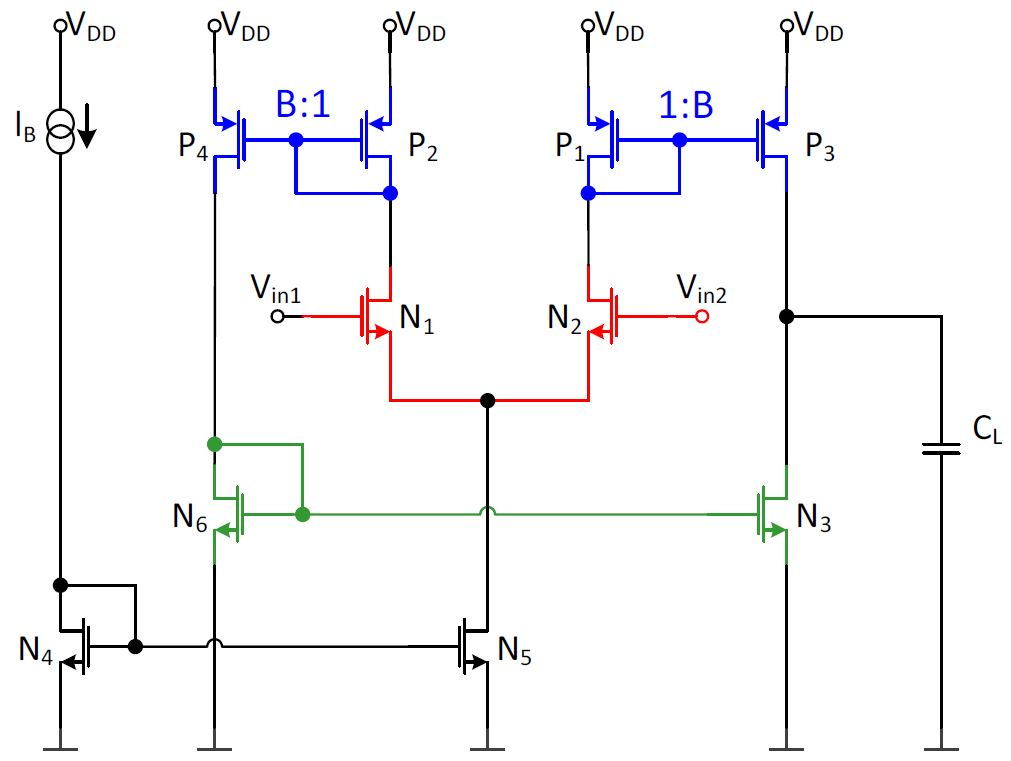
\includegraphics[width=1\linewidth]{chapters/OTA/images/SymmetrischerOTA}\\
\end{minipage}
\begin{minipage}[t]{0.25\textwidth}
	\textbf{Telescopic cascode OTA}\\
	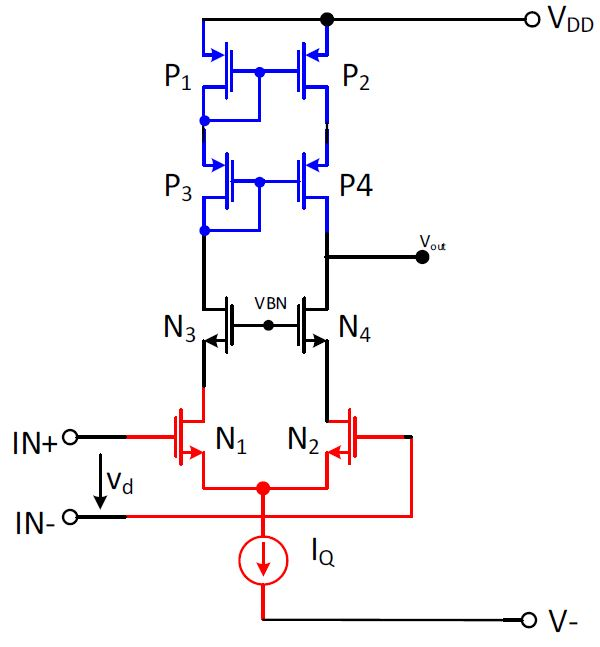
\includegraphics[width=0.7\linewidth]{chapters/OTA/images/TelescopicCascodeOTA}\\
\end{minipage}
\begin{minipage}[t]{0.5\textwidth}
	\textbf{Folded cascode OTA}\\
	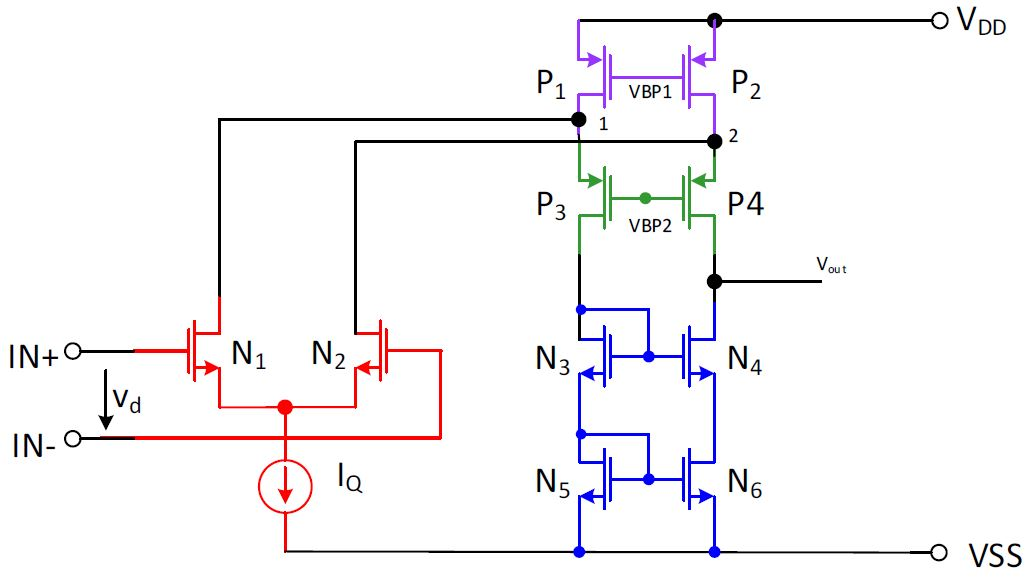
\includegraphics[width=0.7\linewidth]{chapters/OTA/images/FoldedCascodeOTA}\\
\end{minipage}\\
\begin{tabular}{|l|p{3cm}|l|l|l|p{3cm}|}
	\hline
	OTA-Typ&$a$&$r_{out}$&$BW$&$GBW$&Bemerkung\\ \hline
	Symmetrischer OTA&$B\cdot g_{m\_N1}\cdot r_{out}$&$(r_{DS\_N3}||r_{DS\_P3})$&$\frac{1}{2\pi\cdot r_{out}C_L}$&$B\cdot\frac{g_{m\_N1}}{2\pi\cdot C_L}$& \\ \hline
	Telescopic Cascode&$-g_{mN1,N2} \cdot r_{out}$&$(r_{K\_N}||r_{K\_P})$&$\frac{1}{2\pi\cdot r_{out}C_L}$&$\frac{g_{m\_N1,2}}{2\pi C_L}$&$r_{K\_N,K\_P}\approx r_{DS}\cdot(2+g_m\cdot r_{DS})$\\ \hline
	Folded Cascode&$g_{mN1,N2}\cdot r_{out}$&$(r_{K\_N}||r_{K\_P})$&$\frac{1}{2\pi\cdot r_{out}C_L}$&$\frac{g_{m\_N1,2}}{2\pi\cdot C_L}$&\\ \hline
	
\end{tabular}\\[2ex]
\textbf{Miller OTA - Designgleichungen}\\
\begin{minipage}[t]{0.3\textwidth}
	Schaltung:\\
	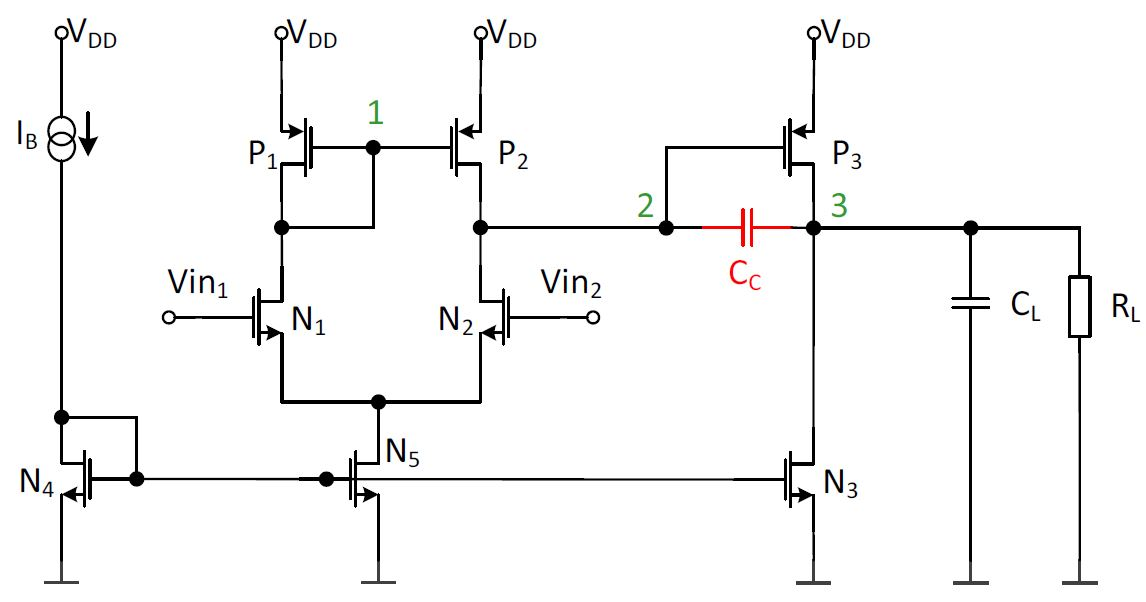
\includegraphics[width=1\linewidth]{chapters/OTA/images/MillerOTA}
\end{minipage}
\begin{minipage}[t]{0.7\textwidth}
	Wichtige Parameter:\\
	\begin{tabular}{|l|l|}
		\hline
		Dominanter Pol:&$f_{pN2}=\frac{1}{2\pi R_{N2}(C_{N2}+a_2C_c)}\approx\frac{1}{2\pi R_{N2}a_2C_c}$\\ \hline
		Nondominanter Pol:&$f_{Nd}=f_{N3}=\frac{1}{2\pi R_{N3}C_L}\approx\frac{g_{mP3}}{2\pi C_L}$\\ \hline
		3dB Bandbreite:&$BW\approx f_d=f_{N2}=\frac{1}{2\pi R_{N2}a_2C_c}$\\ \hline
		Phasenmarge:&$\varphi_M =\SI{90}{\degree}-arctan(\frac{GBW}{f_{nd}})$\\ \hline
		Gain-Bandwidth Produkt:&$GBP=a\cdot f_d=\frac{g_{mN1,2}R_{N2}\cdot g_{mP3}R_{N3}}{2\pi R_{N2}a_2C_c}=\frac{g_{mN1}}{2\pi C_c}$\\ \hline
		Nullstelle:&$f_z\approx\frac{g_{mP3}}{2\pi C_c}$\\ \hline
		Verstärkung:&$a=a_1\cdot a_2=g_{mN1,2}R_{N2}\cdot g_{mP3}R_{N3}=$\\
		&$g_{mN1,2}(r_{DS\_N2}||r_{DS\_P2})\cdot g_{mP3}(r_{DS\_N3}||r_{DS\_N3}||R_L)$\\ \hline
	\end{tabular}
\end{minipage}

% !TeX spellcheck = de_CH_frami
\section{Spannungsreferenzen (Kap. 15)}
In vielen Anwendungen benötigt man eine Spannung, die unabhängig von Betriebsspannungsschwankungen oder Temperaturänderungen ist.
Eine solche Spannungsquelle wird als Spannungsreferenz bezeichnet.\\
\begin{minipage}[t]{0.2\textwidth}
	\textbf{Spannungsteiler}\\
	\includegraphics[height=4cm]{chapters/Spannungsref/images/Spannungsteiler}
\end{minipage}
\begin{minipage}[t]{0.2\textwidth}
	\textbf{MOS-Diode}\\
	\includegraphics[height=4cm]{chapters/Spannungsref/images/MOS-Diode}
\end{minipage}
\begin{minipage}[t]{0.5\textwidth}
	\textbf{Bandgap-Spannungsreferenz}\\
	\includegraphics[height=4cm]{chapters/Spannungsref/images/BandgapRealisation}
\end{minipage}\\
\begin{tabular}{|p{2.4cm}|p{4cm}|l|l|}
	\hline
	&\textbf{Temperatur:}&\textbf{VDD/VSS:}&\textbf{Prozessvariation:}\\ \hline
	Spannungsteiler&S klein&$S = 1$&S klein\\ \hline
	MOS-Diode&S klein&$S < 1$&S: Darf nicht vernachlässigt werden.\\ \hline
	Bandgap&Abhängig von $\Phi_t=\frac{kT}{e}$ und von $R$&0 (unabhängig von VDD/VSS)&Klein\\ \hline
\end{tabular}\\
\subsection{Bandgap-Spannungsreferenz}
In vielen Anwendungen benötigt man eine Spannung, die unabhängig von Betriebsspannungsschwankungen oder Temperaturänderungen ist.
Die Bandgap ist eine Möglichkeit, eine stabile Spannungsreferenz zu erhalten.\\
\begin{minipage}[c]{0.5\textwidth}
	\includegraphics[width=1\linewidth]{chapters/Spannungsref/images/Bandgap}
\end{minipage}
\begin{minipage}[c]{0.5\textwidth}
	\textbf{Formeln:}\\
	$V_{ref} = V_D + K\cdot \Phi_t$\\
	$\Phi_t = \frac{kT}{e}$\\[2ex]
	\textbf{Konstanten:}\\
	$k = \SI{1.38e-23}{\joule / \kelvin}$\\
	T = Absolute Temperatur in K\\
	$e = \SI{1.60e-19}{\coulomb}$\\
	Bei Raumtemperatur ($T=\SI{300}{\kelvin}$ bzw. $\SI{27}{\degreeCelsius}$) ist $\Phi_t = \SI{25.9}{\milli\volt}$
\end{minipage}
% !TeX spellcheck = de_CH_frami

\section{Allgemeines}

\uline{\textbf{Begriffe:}}\\
\begin{minipage}[c]{0.1\textwidth}
	CMOS
\end{minipage}
\begin{minipage}[c]{0.8\textwidth}
	complementary metal oxide semiconductor
\end{minipage}\\[2ex]
\begin{minipage}[t]{0.49\textwidth}
	\uline{\textbf{Grosssignal Ersatzschaltung:}}\\
	Die DC-Ersatzschaltung wird zur Berechnung des Arbeitspunktes, d.h. der Gleichspannungen und Gleichströme benötigt.
	
	\textbf{Grosssignal-Ersatzschaltung bilden}
	\begin{itemize}
		\item Reine AC-Spannungsquellen durch Kurzschlüsse ersetzen, AC-Spannungsquellen mit DC-Anteil durch Gleichspannungsquellen ersetzen
		\item Reine AC-Stromquellen entfernen (d.h. durch Leerläufe ersetzen), AC-Stromquellen mit DC-Anteil durch Gleichstromquellen ersetzen
		\item Kondensatoren entfernen (d.h. durch Leerläufe ersetzen)
		\item Spulen in der Schaltung kurzschliessen (d.h. durch Kurzschlüsse ersetzen)
	\end{itemize}
\end{minipage}
\begin{minipage}{0.02\textwidth}
	
\end{minipage}
\begin{minipage}[t]{0.49\textwidth}
	\uline{\textbf{Kleinsignal Ersatzschaltung:}}\\
	AC- oder Kleinsignalersatzschaltung zur Berechnung der Verstärkungsfaktoren sowie der Ein- und Ausgangswiderstände der Schaltung.
	
	\textbf{Kleinsignal-Ersatzschaltung bilden}
	\begin{itemize}
		\item DC-Spannungsquellen durch Kurzschlüsse ersetzen
		\item DC-Stromquellen entfernen (d.h. durch Leerläufe ersetzen)
		\item Nichtlineare Bauteile durch ihre Kleinsignal-Ersatzschaltungen ersetzen. Das bedeutet vor allem, dass nichtlineare Widerstände durch den Kleinsignalwiderstand, den sie im Arbeitspunkt haben, ersetzt werden müssen.
		\item Koppel- und Bypass-Kondensatoren (d.h. alle Kondensatoren, die wir als gross bezeichnen) kurzschliessen
		\item Sperrdrosseln (d.h. alle Induktivitäten, die wir als gross bezeichnen) entfernen
	\end{itemize}
\end{minipage}









%
\end{document}
